\chapter{Biological Deep Learning}
\chplabel{learning}

The previous chapters of this thesis examined how spiking neural networks
of various depths might be implemented in a biological system.
They did not look at how a biological system might
\emph{learn} such networks.
This chapter looks at the problem of biological learning of deep networks,
specifically the following question:
How does the brain solve the spatial credit assignment problem
to develop deep networks skilled at solving real-world tasks?


\section{Background}

Recently, there has been increased interest from the machine learning community
as to how the brain might learn deep networks
(see \textcite{Marblestone2016} for a review).
One significant difference between these recent efforts
and many previous neuroscientific inquiries into learning
is the distinct emphasis on high-level functionality.
Machine learning researchers are accustomed to
evaluating their algorithms on functional tasks, such as object classification.
Their approach to biological learning is no different,
except that the learning algorithms are designed
to be biologically plausible.
This section first highlights the reasons why
the core of almost all state-of-the-art deep learning systems---%
the backpropagation algorithm---is not biologically plausible (\scn{bp-problems}).
Then, it reviews four ways to overcome this problem,
either by proposing neural mechanisms
that might be able to implement backpropagation (\scn{bp-biomechanisms}),
or by using alternative credit-assignment methods
that avoid the problems faced by backpropagation
(Sections~\scnref{fa-bg}, \scnref{dtp-bg}, and \scnref{ep-bg}).


\subsection{Biological problems with backpropagation}
\scnlabel{bp-problems}

The backpropagation algorithm (BP, see \scn{backprop})
has been very successful for training deep neural networks for many tasks,
including object classification.
Yet there are no known mechanisms by which the brain could implement BP.
\textcite{Bengio2015} list a number of factors
that make BP not biologically-plausible:
\begin{enumerate}
  \item \textbf{The weight transport problem:}
    BP uses the same connection weights
    both for the forwards pass (to perform inference)
    and the backwards pass (to transmit errors back through the network).
    Synapses in the brain are uni-directional,
    with a clear presynaptic and postsynaptic neuron.
    It is unclear how they could be used to transmit errors backwards.
    If a separate backwards connection is posited,
    its strength (connection weight) would need to be synchronized
    with that of the forward connection,
    again something that would be difficult in a biological system.
  \item \textbf{The derivative transport problem:}
    BP relies on the derivative of each hidden unit
    at the current operating point (forward activation).
    Not only is it unclear how this derivative might be computed,
    but it is then used to modulate the error signal,
    which is propagated further back in the network.
    Thus, each neuron needs to be able to use its derivative
    to modulate whatever mechanism is storing/transporting the error signal.
  \item \textbf{The linear feedback problem:}
    In BP, the feedback path is purely linear,
    whereas the biological neurons that would need to implement it are non-linear.
    This could potentially be addressed with population-coding methods
    like the NEF (see \scn{nef}),
    though care would have to be taken such that the number of
    required feedback neurons is within reasonable limits.
  \item \textbf{The spiking problem:}
    BP works with rate-based neurons, while the brain uses spiking neurons.
    While this problem has been partially addressed by the previous chapters
    of this thesis,
    it presents unique problems in the context of online learning,
    particularly since the derivative of a neuron is taken with respect
    to the firing rates (\ie/ filtered spikes), not the spikes themselves.
  \item \textbf{The timing problem:}
    The back-propagation phase of BP uses information
    from the forward-propagation phase.
    Not only is the output of the network used to compute the overall error,
    but both the presynaptic activity (used directly)
    and postsynaptic activity (used to compute the derivative at that node)
    are needed to update the weights.
    This is difficult in a biological deep network,
    because there is delay inherent in each neural connection.
    It takes a significant amount of time for information to propagate
    through the network to provide an output classification
    (which is presumably used to generate the error signal),
    and even more time for this error signal to be propagated back
    to the earliest layers.
    By this time, the activities of the early layers may have changed,
    putting them out of sync with the error signal.
  \item \textbf{The target problem:}
    Most of the success in machine learning for object classification
    has relied on a supervised learning paradigm.
    This assumes that for each training image,
    we know the true category label for that image.
    In the brain, it is not clear where this category label comes from.
    State-of-the-art DNNs learn from millions of images,
    but children only have to be told a handful of times what is a cat, dog, etc.
    The most obvious way for the brain to address this would be to combine
    large amounts of unsupervised learning
    with the small number of provided labels (supervised learning),
    for example to cluster similar input stimuli (\eg/ different cats)
    so that only the cluster has to be labelled, not all the individual stimuli.
    The details of how the brain might execute this semi-supervised learning
    are still largely unknown.
\end{enumerate}
Other than the term ``weight transport'',
which was coined by \textcite{Grossberg1987},
these problem names are first suggested here,
so they are not in common parlance.

One additional problem not pointed out by \textcite{Bengio2015}
is that BP networks do not obey Dale's principle \parencite{Baldi2016},
which states that neurons are almost always either excitatory or inhibitory,
meaning they only release either excitatory or inhibitory neurotransmitters,
not both.
In an abstract neural network,
this means that the signs of connections coming out of a neuron
should either be all positive or all negative, never a mix.
BP does not respect this rule,
and furthermore allows connections to change sign over the course of training,
which is also not biologically realistic.

Another problem not raised by \textcite{Bengio2015}
is how feedforward and feedback signals can combine within a single neuron
to simultaneously allow for feedforward prediction and learning \parencite{Guergiuev2017}.
In BP, there is an error signal associated with each hidden neuron,
determined by backpropagating the error signals of the previous layer
using the forward connection weights.
This error signal modulates learning at all of the afferent synapses of the neuron,
and thus must be injected into the neuron in some way.
The question is: How does this happen,
without mixing with the feedforward signals also entering the neuron?

A distinct but related problem is how the derivative of the neuron activity
might be propagated within the neuron to arrive at the synapses.
Significant research has been done in the area of \emph{backpropagating action potentials},
which are action potentials (spikes) that propagate from a neuron's soma
backwards through the dendrites \parencite{Waters2005}.
It is often hypothesized that these are related to learning,
but there is still a lack of understanding of how they operate,
and how they may propagate backwards without affecting or being affected by
the forwards activity of the dendrites.
These problems compound with the timing problem,
since not only does everything need to arrive in the right place,
it also has to be there at the right time.

In addition to these core problems with BP,
there are many additional problems related to the tools and techniques
typically used when training deep networks in machine learning.
I do not attempt to enumerate them all here,
nor do I address them in this thesis.
Examples include:
architectural problems, such as how neurons might implement
max-pooling or local contrast normalization (or something similar);
initialization problems, such as how connectivity between neurons
is initially established;
and training problems, such as how the brain could implement momentum,
or adjust learning rates
(at the network, layer, or individual neuron level, and possibly over time).
None of these features are necessary for deep learning---%
one can learn, to some degree, with a simple randomly or locally connected
network with no pooling, normalization, or momentum, and a fixed learning rate.
However, current state-of-the-art results in machine learning
typically combine many of these features.

The fundamental goal of this subfield, then,
is to determine how the brain solves the spatial credit assignment problem.
The first approach has been to propose biological mechanisms
by which BP itself could be implemented by the brain,
specifically by finding or positing biological mechanisms
to solve the weight transport problem
(since weight transport seems to be the largest problem with BP,
research has focused on addressing it).
The second approach is to look for alternative credit assignment methods,
again often starting with weight transport as the fundamental problem,
and once it has been solved,
expanding the method to address the other problems with BP as well.
A third approach is to reject the problem entirely,
by positing that the brain does not solve the credit assignment at all.
The new problem is then to explain how the brain might learn
to perform complex tasks
using only shallow supervised learning, unsupervised learning,
and other methods that do not rely on performing spatial credit assignment;
this lies outside the scope of this thesis.
Likely, the final answer will lie somewhere within all three of these approaches,
taking elements of BP and combining them both with
novel credit assignment strategies and other learning methods.


\subsection{Biological mechanisms for backpropagation}
\scnlabel{bp-biomechanisms}

\textcite{Bogacz2000} was one of the first papers to try to address
some of the biological plausibility limitations of BP.
The main contribution of the paper is that they perform a type of learning
with some similarities to BP
in a spiking neural network with a hidden layer.
However, their method is specific to a very constrained type of network.
The purpose of the network is to determine whether a stimulus is novel
or has been previously presented to the network (familiar).
If presented with a novel stimulus, the network updates
using a one-shot-learning paradigm so that the stimulus
will subsequently be classified as familiar.
The structure of this network has one hidden layer.
The connection weights from the input to the hidden layer are learned,
but the output neuron simply sums across the hidden neurons
and thresholds the response.
Credit assignment in this structure is much easier than in a general network,
since all hidden neurons contribute equally to the output,
while BP in a general network would need
to propagate the error backwards through variable connection weights
from the hidden neurons to the output.
The authors acknowledge this,
and identify the generalization to variable-weight outputs as future work.
This generalization (\ie/ solving the weight transport problem) is not straightforward,
and has been the focus of much of the subsequent work on
biologically plausible credit assignment.


\subsection{Feedback Alignment (FA)}
\scnlabel{fa-bg}

Feedback Alignment (FA) \parencite{Lillicrap2014}
is an alternative to BP for biological credit assignment.
The idea behind FA is that the feedback weights---%
the weights used to transmit error information backwards through the network---%
do not need to be the transpose of the feedforward weights ($W^T$),
as they are in BP.
Instead, FA uses random feedback weights,
and finds that the feedforward weights ``align'' themselves
so that useful error information can be propagated backwards through the network.
Specifically, the feedforward weights align themselves so that they are
not orthogonal to the feedback weights,
thus allowing the feedback error signals to push the neuron activities
in a direction that somewhat decreases the overall error
(despite not being the optimal, \ie/ gradient, direction).

% Poggio paper that says signs need to be the same
\textcite{Liao2015} focus on the weight transport problem,
and find that networks perform better when there is concordance between
the signs of the feedback weights and the feedforward weights.
This is perhaps not surprising,
since having feedback weights with the same signs as the feedforward weights
makes it highly likely that the two sets of weights will be far from orthogonal,
and thus the feedback weights will transmit useful information.
They also find that using some sort of batch normalization \parencite{Ioffe2015}
is very beneficial for any learning method where the feedback weights
are not the transpose of the feedforward weights
(which they broadly call ``asymmetric backpropagation'').
When training ANNs, weights may change sign during training,
so at first blush sign concordance may seem to not be biologically plausible,
since it could again require symmetry between feedforward and feedback weights
(albeit a more relaxed form of symmetry).
However, connections in the brain do not change sign over time;
they are all either inherently excitatory or inhibitory.\footnote{
  In fact, the constraint is even stronger:
  each \emph{neuron} only either has excitatory or inhibitory efferent connections.
  This is known as Dale's Principle.}
My conclusion is that sign changes over time do not pose a threat to possible
sign concordance in the brain,
though additional issues would have to be addressed
to concretely demonstrate its biological plausibility.
(I am not aware of a large-scale learning system
that obeys Dale's principle in the feedforward connections,
never mind one that would also obey both Dale's principle and sign concordance
in the feedback path.)

% Application of direct FA
\textcite{Nokland2016} uses FA to tackle some more difficult datasets---%
namely CIFAR-10 and CIFAR-100---as well as MNIST.
On MNIST, FA and its \emph{direct FA} variant (DFA, see \scn{fa-variants})
perform almost as well as BP across a number of different network architectures.
This paper also investigates a very deep network (with 100 layers of 240 tanh units each),
for which only DFA is able to converge,
presumably because it helps mitigate
the vanishing and exploding gradient problems.\footnote{
  However, the average test-set error (3.92\%) for this architecture
  is worse than for simpler architectures,
  including a 7-layer network (2.32\%)
  and a single-layer network with 800 tanh units (1.68\%).}
On CIFAR-10 and CIFAR-100,
FA and DFA are able to perform within a few percentage points
of BP on the test set for fully-connected networks.
For convolutional networks, FA and DFA perform significantly worse than BP
(27.1\% and 26.9\% vs 22.5\% respectively on CIFAR-10).
This could be because convolutional networks have fewer parameters,
meaning less redundancy,
and FA typically needs more parameters than BP
since the fixed random feedback weights
constrain the space that any particular neuron can explore during learning
(see \scn{fa-limitations-results}).
Finally, the paper introduces a novel FA variant called \emph{indirect FA},
which uses random direct feedback to the first hidden layer,
then forward connections to propagate this error forward (see \scn{fa-variants}).
There are some biological reservations to this approach, however,
since the forward connections skip the neural nonlinearity
and only use the connection weights.
No results from the IFA algorithm are presented.

\textcite{Baldi2016} perform more in-depth analyses on the FA algorithm,
both theoretical and experimental.
One of their key results is that FA is ``very robust
and works almost as well as BP'', and that
``performance is unaffected or degrades gracefully
when the the random backwards weights are initialized from different
distributions or even change during training.''
They perform experiments that look at varying levels of sparsity
in the feedback weights,
and find that FA achieves the same test error on MNIST
for sparsity levels from 20\% to 80\% (where non-zero elements all equal one).
Additionally, they test FA on a convolutional CIFAR-10 architecture,
and are able to achieve around 25\% test-set error
(their reference BP implementation achieves 16\%).
In addition to the tests on existing FA variants,
they introduce two novel FA variants,
which they call \emph{adaptive random backpropagation (ARBP)}
and \emph{adaptive skipped random backpropagation (ASRBP)}.
They operate the same as FA and DFA, respectively,
except that the feedback channels are also allowed to learn over time.
They do not perform extensive tests of these algorithms,
but a test on MNIST shows that ASRBP speeds up training slightly
as compared with its non-adaptive counterpart.
ARBP also works, but is much more fragile,
requiring a much smaller learning rate on the backwards connections,
and even then showing a non-smooth error trajectory.

\textcite{Neftci2017} implement a spiking version of direct FA
targeting neuromorphic hardware.
One major innovation over the \textcite{Lillicrap2016} spiking FA model
is that they do not use the exact neural derivative,
but rather use a surrogate derivative function
to approximate the neural derivative.
This allows them to train with LIF neurons.
They also introduce a form of probabilistic regularization
where spikes are randomly dropped based on a given probability;
this slightly improves test-set results.
The algorithm is event-driven,
meaning that weights are only updated when the corresponding presynaptic neuron spikes.
They demonstrate their spiking training method on MNIST,
and show that the final network can achieve 2.25\% test-set error.
Using a first-to-spike classification method yields around 4.5\% test-set error
while using 50 times less power than the better classification method.

\textcite{Samadi2017} also implement a spiking version of direct FA
(which they call broadcast alignment, or BA) in LIF neurons.
To approximate the LIF neuron derivative,
they fit the LIF rate-response curve with the following function:
\begin{align}
  f(x) = \max(0, c_1 \tanh(c_2 x)) \text{ ,}
\end{align}
where $x$ is the neuron input (current)
and $c_1$ and $c_2$ are arbitrary constants (hyperparameters).
This function fits the LIF rate-response curve reasonably well,
and is everywhere differentiable.
Using this as a surrogate derivative function,
they are able to train spiking networks to achieve 2.95\% test-set error on MNIST.
Their comparable rate-based networks achieve
1.40\% error with BP, 1.78\% with FA, and 2.36\% with DFA.


\subsection{Difference Target Propagation (DTP)}
\scnlabel{dtp-bg}

\newcommand{\vh}{\vect{h}}
%% $\hat \vh$

Difference Target Propagation (DTP) \parencite{Lee2015a}
is another algorithm for solving the spatial credit assignment problem
in a biological system.
Rather than using random feedback weights (as FA)
or symmetric feedback weights (as BP),
it \emph{learns} feedback weights to propagate error information.
The objective for the backwards path is to learn an approximate inverse $g^i$
for the forward function $f(\vh^{i-1}) = \vh^i = F^i(W^i \vh^{i-1})$
computed by the weights $W^i$ and neural nonlinearity $F^i$ at each layer.
Using this approximate inverse, we can compute a ``target'' value $\hat \vh^i$
for a layer given the target value $\hat \vh^{i+1}$ for the subsequent layer
\begin{align}
  \hat \vh^i = \vh^i + g^{i+1}(\hat \vh^{i+1}) - g^{i+1}(\vh^{i+1}) \text{ .}
  \eqnlabel{dtp}
\end{align}
This equation is designed so that when $\hat\vh^{i+1} = \vh^{i+1}$,
then $\hat\vh^i = \vh^i$.
This ensures that when there is no error at the highest layer,
then learning stops throughout the system.
The more intuitive choice of $\hat\vh^i = g^{i+1}(\hat\vh^{i+1})$---%
that is, simply propagating the target backwards---%
obeys this same property if $g^i$ is the inverse of $f^i$,
but not if $g^i$ is only an approximation of the inverse of $f^i$,
hence the choice of the more complicated \eqn{dtp}.
The target for the final layer is computed as a small step
in the direction of the gradient for that layer:
\begin{align}
  \hat \vh^N = \vh^N - \hat\eta \pdiff{O(\vh^N, y^*)}{\vh^N} \text{ .}
\end{align}
DTP can learn relatively deep networks;
the authors use it to learn a network with 7 hidden layers of 240 units each
on MNIST, achieving 1.94\% error using tanh units (compare 1.86\% for BP).
Interestingly, the same network with ReLU units
achieved 3.15\% with DTP, whereas BP achieved 1.62\%.
The authors also tested a network on CIFAR-10,
achieving 50.71\% with DTP versus 53.72\% for BP;
these numbers are good for a fully connected network without data augmentation.

% Towards deep learning with segregated dendrites
% - Explains how feedforward and feedback error can combine in one neuron
Although DTP offers a solution to the weight transport
and linear feedback problems,
it is unclear how exactly the feedback connections would operate
in a biological network.
There are two concerns:
1) each feedback connection is used to transmit two distinct values,
$g^i(\hat\vh^i)$ and $g^i(\vh^i)$,
it is unclear how they could be transmitted simultaneously;
2) the feedback connection $g^i$ needs to receive both
$\hat\vh^i$ and $\vh^i$ as input,
thus they must be stored in the same place,
but it is unclear how a single neural population
could store both feedforward ($\vh^i$) and feedback error ($\hat\vh^i$)
signals.
\textcite{Guergiuev2017} extend the DTP algorithm
with a compartmental neuron model,
addressing both of these questions.
Their hidden neurons have three compartments:
an apical dendrite that accepts feedback connections;
a basal dendrite that accepts feedforward connections;
and a soma, which receives input from both dendritic compartments
and controls the neuron's output.
There are two distinct phases to each stimulus presentation:
a forward phase, where the forward activity is computed;
and a target phase, where the correct category signal
is applied at the top layer.
This allows the model to compute ``plateau potentials'' $\alpha^f$ and $\alpha^t$
in the apical dendrites;
these signals are analogous to $g^i(h^i)$ and $g^i(\hat h^i)$
in DTP, respectively.
The output of each neuron is a firing rate,
determined by applying a sigmoid function to the soma's membrane voltage.
They demonstrate that a two-layer version of their model
is able to learn on MNIST,
achieving 3.2\% test-set error.


\subsection{Equilibrium Propagation (EP)}
\scnlabel{ep-bg}

Ten years ago, \textcite{Hinton2007} proposed the idea that
neurons could use derivatives in activity to transmit error information.
The general idea is that after the forward pass,
the top-level neurons in the network are perturbed
to push them closer to the target output values (as in DTP).
This change in activity over time codes for the error gradient of those neurons;
this is then propagated backwards
(using symmetric weights in Hinton's original proposition).
This would explain how neurons seemingly transmit both
forward signals and error information within a short span of time.
It could also help explain the spike-timing-dependent plasticity (STDP)
curves that \textcite{Bi1998} first identified empirically.

More recently, \textcite{Bengio2015} began to try to embody these ideas
into a quantitative model,
to demonstrate that they could actually work in practice.
This first paper presented a generative statistical model
utilizing the temporal derivative idea,
which was able to fill in corrupted sections of MNIST digits.

\textcite{Bengio2017} present an alternate use for the
derivative error encoding idea,
to perform inference in an energy-based model with symmetric weights.
They demonstrate that such a model reproduces STDP-like curves
in the weight changes.
\textcite{Scellier2017} extend this idea to a deep network
that is able to learn to perform the MNIST task,
achieving 0.0\% training error for all three networks tested
and between 2\% and 3\% test error depending on the number of layers used.
They title this algorithm Equilibrium Propagation (EP).
The model has two distinct phases:
an inference phase, where the model settles to a steady-state
given a stimulus;
and an error propagation phase,
where the energy is increased slightly based on the error of the network output,
and the model settles to a new steady-state minimizing
the combined energy from the stimulus and output error.
Weight changes are Hebbian,
based on the new (stimulus and label) steady-state activities,
and anti-Hebbian, based on the stimulus-only steady-state.
This pushes the model to associate lower energy
with the correct stimulus-label pairs.

This tentative connection between derivatives of neuron activity,
error, and STDP is very intriguing from a biological perspective,
since it would explain how neurons
are able to encode both activities for inference from the stimulus
and the error or correction information needed to learn.
The energy-based approach is also enticing,
since it quantitatively describes how an arbitrarily-connected neural system
can perform inference over time given a stimulus.
This opens the door for recurrent or lateral connections
that allow for a more complex inference process over time,
rather than just the simple feedforward inference used by
most current object-classification networks.\footnote{
  It also introduces more considerations,
  first and foremost the amount of time needed by a network
  with recurrent and lateral connectivity to settle to a steady-state.}
While these models do make these ideas more concrete,
there are still open questions about how they could work biologically.
The most significant one is again the weight transport problem;
the energy-based models re-introduce symmetric connections,
bringing back all the problems that other approaches
have explicitly worked to overcome.
While \textcite{Scellier2017} is hopeful that this can be overcome---%
making analogies to how autoencoders were able to move to using untied weights,
and how FA has addressed the need for symmetric weights in BP---%
it is still unclear how this might be addressed in an energy-based model.
The other biological consideration with these models is the timing aspect:
they involve distinct inference (no label information)
and clamped (label information provided) phases,
and in the case of \textcite{Scellier2017} these phases
are quite different lengths.
It is unclear how the brain might coordinate between such phases,
especially since the weight updates require neural activities
from both phases.

% - Could STDP be responsible for the anti-Hebbian/Hebbian switch, such that
%   the learning rule would only work properly when implemented in spiking neurons?
% - What about settling time? How could this be controlled?
% - Can this be combined with ideas from FA or DTP, such that symmetric back
%   weights are not required?
% - Can skip connections help reduce settling time? If I can get some class
%   information from the first hidden layer, this could help prime later layers


\section{Feedback Alignment}
\scnlabel{fa-methods}

Feedback Alignment (FA) is an alternative credit assignment method
first proposed by \textcite{Lillicrap2014};
since then, the core idea has been studied by a number of other researchers,
sometimes under the name Random Backpropagation (RBP) \parencite[\eg/][]{Liao2015,Baldi2016,Nokland2016}.

As mentioned in \scn{fa-bg},
the core idea of the algorithm is to use the same network structure as BP,
but to use static random feedback weights
(rather than the transpose of the forward weights)
during the backwards pass.\footnote{
  See \scn{backprop} for a presentation of the backpropagation (BP) algorithm.
  Some of the notation used in this section is defined there.}
This solves the weight transport problem,
since the feedback weights do not need to be kept identical to the feedforward ones.
Some variants of the algorithm (explored in \scn{fa-variants})
also address the derivative transport problem.
Finally, \textcite{Lillicrap2016} constructed a spiking version of their network
that also addresses the linear feedback, spiking, and timing problems
to varying degrees.

The success of the FA algorithm---%
and even the fact that it is able to learn anything at all---%
has surprised many researchers.
It seems counter-intuitive that back-propagating a random projection
of the subsequent layer's error
would transmit any useful information.
At first blush, it seems that the random projection would make the errors random:
uncorrelated to the output errors and thus uninformative and useless.
The first part of this intuition is correct:
the errors are in fact random.
However, since the random projections are fixed,
there is still structure to the errors,
and their values contain information about the nature of the output error.
To better understand how FA allows for learning,
it is important to develop intuitions about how the algorithm works.


\subsection{Intuitions}
\scnlabel{fa-intuitions}

% ``alignment'' intuition
% - Explain why this should happen. Hidden neurons are being pushed to be
%   selective for certain classes, so forward classification weights will match
The first intuition about FA is what I will call the ``alignment'' intuition.
It was presented as part of the original FA paper \parencite{Lillicrap2014},
and is where the name ``feedback alignment'' comes from.
The intuition is that over time, the forward weights in an FA network
will ``align'' themselves so they are not orthogonal with the backwards weights.\footnote{
  Here, two matrices $\mat A$ and $\mat B$ are essentially orthogonal
  if the images of these matrices across error vectors $\vect e$
  is approximately orthogonal:
  $\vect e \mat B \mat A^T \vect e^T \approx 0$ for all $\vect e$.
  In practice, FA works as long as $\vect e \mat B \mat W \vect e^T > 0$
  for most error vectors $\vect e$,
  where $\mat W$ is our forward weight matrix
  and $\mat B$ is our random feedback weight matrix \parencite{Lillicrap2014}.
  To assess this, we can look at the eigenvalues of $\mat B \mat W$:
  if they all have positive real components,
  then the dot product in the previous expression will be positive for all $\vect e$.}
If the forwards and backwards weights are orthogonal,
then the projected error will not provide any useful information
to help correct the actual errors of the network.
Put another way, the change in the network weights
will be orthogonal to the gradient,
and thus not decrease the error.\footnote{
  It is important to note that this explanation assumes linear neurons,
  but the same ideas apply in the case of nonlinear neurons.}
As soon as the feedback weights are non-orthogonal (in a positive direction)
with the feedforward weights,
then each update will move at least partially in the same direction as the gradient,
that is, in a direction that decreases the error.
The smaller the angle between the feedforward and feedback weight matrices,
the more similar the update is to the gradient,
and the more the error will decrease with each step.
If the angle is zero, then the feedback weights are the transpose of the feedforward,
and we move in the direction given by BP.
\textcite{Lillicrap2014} presented this as the motivating idea behind FA,
and found empirically that in an FA network,
the angle between the feedforward and feedback matrices
reduces to much less than 90\degree/ (typically less than 45\degree/ in their networks).

So why does this ``alignment'' happen?
To explain this, I introduce a second intuition:
the random feedback matrices push each hidden neuron
to be selective to certain classes and not others.
For example, for the final hidden layer,
each neuron has a randomly-weighted feedback connection to each output error neuron.
If a neuron happens to have a strong positive feedback connection to class A,
then each time a stimulus of class A is presented but not correctly classified
(such that the output error is large),
then that neuron will be pushed to be more active.
It thereby develops an affinity for stimuli of class A.
The reverse process can happen if the neuron has a strong negative connection
to class B; the neuron will learn to be silent for class B stimuli.
Thus, the neuron develops a selectivity for some classes over others.
Once this selectivity begins to form,
then the \emph{feedforward} connections
between that neuron and those classes will strengthen,
since activity in that neuron is indicative of those classes.
In this manner, the neuron will develop both strong positive feedback
and feedforward connections for some classes,
and strong negative ones for other classes.
This makes the feedforward weights more similar to the feedback weights,
causing them to align.

A third intuition is that this push for class selectivity
only happens when there is error in the network output.
An error causes neurons to learn to respond more strongly to the problematic stimulus.
The most change occurs for neurons with a significant derivative
at their current activity level,
since this derivative modulates the learning (see \scn{fa-variants}).
The initial forward connections in the network are random,
and thus some neurons are slightly predisposed from the start
to respond to some stimuli over others.
These factors, when combined with the random feedback weights,
result in hidden neurons that learn to form distributed representations
across all classes and stimuli in the dataset.
Different neurons are responsible for different classes,
and different groups of stimuli within a class.


\subsection{Variants}
\scnlabel{fa-variants}

\begin{figure}
  \centering
  \tikzstyle{line} = [draw]

\begin{tabular}{c|c|c}
  GFA & LFA & DFA \\
\begin{tikzpicture}[->,>=stealth',auto,node distance=2cm,
    thick,circnode/.style={circle,draw,inner sep=2,minimum size=1cm}]

  \node[circnode] (h) {$h^n$};
  \node[circnode] (ha) [above of=h] {$h^{n+1}$};
  \node[circnode] (hb) [below of=h] {$h^{n-1}$};
  \node[circnode] (e) [right of=h, node distance=2.5cm] {$e^n$};
  \node[circnode] (ea) [above of=e] {$e^{n+1}$};
  \node[circnode] (eb) [below of=e] {$e^{n-1}$};

  \path[line] (hb) -- node [right] (Wb) {$W^n$} (h);
  \path[line] (h) -- node [right] (Wa) {$W^{n+1}$} (ha);
  \path[line] (ea) -- node [right] (Ba) {$B^{n+1}$} (e);
  \path[line] (e) -- node [right] (Bb) {$B^n$} (eb);

  \path[line] (h) -- node {$h'$} (e);
  \path[line] (ha) -- node {$h'$} (ea);
  \path[line] (hb) -- node {$h'$} (eb);
  %% \path[line] (h) to [out=30,in=150] node {$h'$} (e);
  \path[line] (ea) to (Wa);
  \path[line] (e) to (Wb);

  \node[] (h0) [below of=hb, node distance=10mm] {};
  \node[] (h1) [above of=ha, node distance=10mm] {};
  \path[line] (h0) -- (hb);
  \path[line] (ha) -- (h1);
  \node[] (e0) [below of=eb, node distance=10mm] {};
  \node[] (e1) [above of=ea, node distance=10mm] {};
  \path[line] (e1) -- (ea);
  \path[line] (eb) -- (e0);
  \node[] (h00) [right of=h0, node distance=10mm] {};
  \path[line] (eb) -- (h00);
\end{tikzpicture}
&
\begin{tikzpicture}[->,>=stealth',auto,node distance=2cm,
    thick,circnode/.style={circle,draw,inner sep=2,minimum size=1cm}]

  \node[circnode] (h) {$h^n$};
  \node[circnode] (ha) [above of=h] {$h^{n+1}$};
  \node[circnode] (hb) [below of=h] {$h^{n-1}$};
  \node[circnode] (e) [right of=h, node distance=2.5cm] {$e^n$};
  \node[circnode] (ea) [above of=e] {$e^{n+1}$};
  \node[circnode] (eb) [below of=e] {$e^{n-1}$};

  \path[line] (hb) -- node [right] (Wb) {$W^n$} (h);
  \path[line] (h) -- node [right] (Wa) {$W^{n+1}$} (ha);
  \path[line] (ea) -- node [right] (Ba) {$B^{n+1}$} (e);
  \path[line] (e) -- node [right] (Bb) {$B^n$} (eb);
  \path[line] (ea) to (Wa);
  \path[line] (e) to (Wb);

  \node[] (h0) [below of=hb, node distance=10mm] {};
  \node[] (h1) [above of=ha, node distance=10mm] {};
  \path[line] (h0) -- (hb);
  \path[line] (ha) -- (h1);
  \node[] (e0) [below of=eb, node distance=10mm] {};
  \node[] (e1) [above of=ea, node distance=10mm] {};
  \path[line] (e1) -- (ea);
  \path[line] (eb) -- (e0);
  \node[] (h00) [right of=h0, node distance=5mm] {};
  \path[line] (eb) -- (h00);

  \path[line] (h.east) .. controls +(right:7mm) and +(up:5mm)
                        .. node [above right] {$h'$} (Wb.north);
  \path[line] (ha.east) .. controls +(right:5mm) and +(up:5mm)
                        .. node [above right] {$h'$} (Wa.north);
  \path[line] (hb.east) .. controls +(right:5mm) and +(up:5mm)
                        .. node [above right] {$h'$} (h00.north);
\end{tikzpicture}
&
\begin{tikzpicture}[->,>=stealth',auto,node distance=2cm,
    thick,circnode/.style={circle,draw,inner sep=2,minimum size=1cm}]

  \node[circnode] (h) {$h^n$};
  \node[circnode] (ha) [above of=h] {$h^{n+1}$};
  \node[circnode] (hb) [below of=h] {$h^{n-1}$};
  \node[circnode] (e) [right of=h, node distance=2.5cm] {$e^n$};
  \node[circnode] (ea) [above of=e] {$e^{n+1}$};
  \node[circnode] (eb) [below of=e] {$e^{n-1}$};
  \node[circnode] (es) [right of=e, node distance=2cm] {$e^*$};

  \path[line] (hb) -- node [right] (Wb) {$W^n$} (h);
  \path[line] (h) -- node [right] (Wa) {$W^{n+1}$} (ha);
  \path[line] (es) -- node [above right] (Bc) {$B^{n+2}$} (ea);
  \path[line] (es) -- node [below] (Ba) {$B^{n+1}$} (e);
  \path[line] (es) -- node [below right] (Bb) {$B^n$} (eb);

  \node[] (h0) [below of=hb, node distance=10mm] {};
  \node[] (h1) [above of=ha, node distance=10mm] {};
  \path[line] (h0) -- (hb);
  \path[line] (ha) -- (h1);
  \node[] (h00) [right of=h0, node distance=5mm] {};

  \path[line] (ea) to (Wa);
  \path[line] (e) to (Wb);
  \path[line] (eb) -- (h00);

  \path[line] (h.east) .. controls +(right:7mm) and +(up:5mm)
                        .. node [above right] {$h'$} (Wb.north);
  \path[line] (ha.east) .. controls +(right:5mm) and +(up:5mm)
                        .. node [above right] {$h'$} (Wa.north);
  \path[line] (hb.east) .. controls +(right:5mm) and +(up:5mm)
                        .. node [above right] {$h'$} (h00.north);
\end{tikzpicture}

\end{tabular}

  \captionb{Diagrams of the three main variants of FA.}{
    Global-derivative FA (GFA, left) has an identical structure to BP,
    but replaces the transpose weights with random weights: $(\mat W^n)^T \to \mat B^n$.
    Local-derivative FA (LFA, middle) is similar to GFA,
    but only applies the neuron derivatives $h'$ locally.
    Direct FA (DFA, right) projects the error signals
    directly from the output error $e^*$.
    Since both the LFA and DFA feedback pathways are linear,
    feedback matrices $\mat B$ can be chosen such that they are equivalent.
  }
  \figlabel{fa-variants}
\end{figure}

There are a number of different variants of the FA algorithm,
as mentioned in \scn{fa-bg}.
For all the variants, the structure of the weight update is the same:
\begin{align}
  \Delta W^n_{ij} &= -\eta e_j^n f'(a_j^n) h_i^{n-1} \text{ .}
\end{align}
That is, all variants use the activity of the presynaptic neurons $h_i^{n-1}$,
the derivative of the postsynaptic neuron activity $f'(a_j^n)$,
and a modulatory error signal $e_j^n$ (and the learning rate $\eta$).
Additionally, the output layer performs shallow learning in all variants,
as in BP:
\begin{align}
  \Delta W^{N+1}_{ij} = -\eta e^*_j h_i^N
\end{align}
where $e^*_j = y_j - y^*_j$ and $N$ is the number of hidden layers in the network.
What changes between variants is how the feedback error signal $\vect e^n$
is determined,
that is, the structure of the feedback chain.
\fig{fa-variants} shows diagrams of the three main variants
examined in this thesis.

The original FA algorithm from \textcite{Lillicrap2014}
uses the neuron derivatives as part of the feedback chain;
I call this \emph{global-derivative FA} (GFA).
Its key feature is that it uses the hidden-neuron derivatives in the feedback chain:
\begin{align}
  e^n_j = \sum_q e^{n+1}_q f'(a^{n+1}_q) B^{n+1}_{qj} \text{ .}
\end{align}
Here, $\mat B^{n+1}$ is the matrix of random feedback weights
that projects the error from the space of layer $n + 1$ to the space of layer $n$.\footnote{
  All variants of FA include random feedback weight matrices $\mat B$,
  though the dimensionality of the matrices may differ between variants.}
Therefore, the update to the weights $W^n_{ij}$
depends not only on the local postsynaptic derivative $f'(a_j^n)$,
but also on the hidden neuron derivatives from all subsequent layers
(where the exact dependence is determined by the connectivity of the $\mat B$ matrices).

The first variant removes the neuron derivatives from the feedback chain,
and only uses each derivative locally for updating the weights
going into the corresponding neuron.
I call this \emph{local-derivative FA} (LFA);
it can be formulated as follows:
\begin{align}
  e^n_j = \sum_q e^{n+1}_q B^{n+1}_{qj} \text{ .}
\end{align}

The second variant---\emph{direct FA} (DFA)---builds off the fact that
the local-derivative FA passes the error signal at the classification layer $\vect e^*$
through subsequent random linear projections to produce $\vect e^n$.
Assuming no layer has fewer hidden neurons
than the number of output dimensions of the network
(such that no information is lost about $\vect e^*$),
we can achieve a very similar effect by simply projecting each layer's error
signal randomly off the output error signal:
\begin{align}
  e^n_j = \sum_l e^*_l B^{n+1}_{lj} \text{ .}
\end{align}
This variant was proposed both by \textcite{Lillicrap2016} and \textcite{Nokland2016}.
It is also explored by \textcite{Baldi2016},
who call it \emph{skipped random backpropagation}.

A third variant---called \emph{indirect FA} (IFA)---was proposed by \textcite{Nokland2016}.
They present this variant in the context of a two-hidden-layer network.
The first hidden layer receives random feedback from the output layer,
just as with DFA:
\begin{align}
  e^1_i = \sum_l e^*_l B^*_{li} \text{ .}
\end{align}
The second hidden layer's error is based on that of the first layer,
using the input weights of the second layer:
\begin{align}
  e^2_j = \sum_i e^1_i W^2_{ij} \text{ .}
\end{align}
While perhaps somewhat interesting theoretically,
there are reasons to have reservations about using it as a biological model.
The main reservation is that it uses the connection weights
between the first and second hidden layers ($\mat W^2$),
but the error $\vect e^1$ that is projected through these weights
is not integrated by the second hidden-layer neurons
(\ie/ their activity is not affected),
and conversely the error signal is not affected by the neural nonlinearity.
The neuron would need some mechanism such that the error signal
only reaches the synapses and is not passed on to the soma,
while the feedforward currents---passing through the same synapses---%
would pass through to the soma as usual.
Since there is no mechanism to distinguish between electrical currents
in this manner, this poses a significant problem with this method.\footnote{
  The problem of how to manage feedforward and error signals in the same
  cell is common to all variants of Feedback Alignment,
  and learning more generally.
  However, in the other variants,
  feedforward and error signals would only
  co-occur in the postsynaptic neuron's dendrites,
  and would not require passing error information from
  the presynaptic neuron to the postsynaptic neuron through synapses,
  as required by IFA.}
Additionally, it is unclear how this method would generalize
to more than two hidden layers.
If we were to use the third hidden layer's weights to project $\vect e^2$,
then we again run into the problem that we are making use
of the second layer's synapses while avoiding the neural nonlinearity.
Due to these reservations,
combined with the fact that \textcite{Nokland2016}
provided no advantages for the IFA variant,
this thesis does not examine IFA any further.

It is also possible to have learning in the backwards channel,
called \emph{adaptive} FA.
\textcite{Baldi2016} introduce weight changes for their backwards weights
that are proportional to the product of the forward activities
for the layer in question,
as well as the randomly projected error for the previous layer:
\begin{align}
  \Delta B^n_{ij} = \eta\mu \delta^n_i h^{n-1}_j
\end{align}
where $\delta^n_i = e^n_i f'(a^n_i)$,
$\eta$ is the learning rate for the forward weights,
and $\mu$ is a scaling factor on $\eta$ to determine the feedback learning rate.
This is the same update as is applied to the forward weights;
for that reason, I will call it \emph{symmetric} adaptive FA.
A similar update can be applied to DFA:
\begin{align}
  \Delta B^n_{lj} = \eta\mu e^*_l h^{n-1}_j \text{ .}
\end{align}
The idea of adaptive FA is intriguing,
since it can potentially allow initially random feedback weights
to better align with the forward weights,
resulting in better error information transmission
and therefore faster convergence and better performance.
It may also increase the biological plausibility of the model,
since it is unclear whether the brain could maintain static feedback connections
over long periods of time,
particularly when the adjacent forward connections are learning.
In the case of symmetric adaptive FA,
it does also raise the biological question
as to how the forward activities come to modulate the backwards weights.
\textcite{Baldi2016} present only preliminary results on adaptive variants
of both GFA and DFA,
but find that in the case of DFA,
adding adaptation improves convergence and overall performance,
whereas introducing it to GFA makes the algorithm unstable
(even for $\mu = 0.1$).

I am not aware of any other published investigations
into adaptive variants of FA.
Here, I propose two new adaptive variants based on Hebbian learning:
one using a pure Hebbian learning rule;
and the other using Oja's rule \parencite{Oja1982},
a more stable variant of Hebbian learning.
These adaptive variants can be viewed as unsupervised forms of adaptation,
whereas symmetric adaptive FA is more like supervised learning
(where the forward path is providing the teaching signal).
Hebbian ADFA is given by:
\begin{align}
  \Delta B^n_{lj} = \eta\nu e^*_l e^{n-1}_j
\end{align}
where $\eta$ is the forward learning rate
and $\nu$ is a scaling factor on this learning rate.
Oja ADFA is given by:
\begin{align}
  \Delta B^n_{lj} = \eta\nu \left[
    e^*_l e^{n-1}_j - \beta B^n_{lj} \left(e^{n-1}_j\right)^2 \right]\text{ ,}
\end{align}
where $\beta$ is a scaling parameter
to control the amount of regularization (often just set to unity).
These adaptation rules can be combined with symmetric ADFA
to create hybrid rules:
Symmetric Hebbian (Symm-Hebb) ADFA;
and Symmetric Oja (Symm-Oja) ADFA.
These learning rules use a linear weighting of the $\Delta\mat B$ updates
\begin{align}
  \Delta\mat B^n_\text{Symm-Hebb} = &
    \eta\mu \Delta\mat B^n_\text{Symm} + \eta\nu \Delta\mat B^n_\text{Hebb} \\
  \Delta\mat B^n_\text{Symm-Oja} = &
    \eta\mu \Delta\mat B^n_\text{Symm} + \eta\nu \Delta\mat B^n_\text{Oja} \text{ .}
\end{align}
Typically, we will have $\mu = 1$ and $\nu = 0.1$,
giving more weight to the ``supervised'' portion of the rule.


\subsection{Comparison of variants}

Given these three different implementations of the FA algorithm
(GFA, LFA, and DFA),
how should we choose which one to use?
There are two key considerations: performance and biological plausibility.
In \scn{fa-variants-results},
I compare the performance of the different variants,
and find that all the variants perform similarly,
with perhaps the direct variant performing slightly better.

In terms of biological plausibility,
we must consider both how the neuron derivatives are used
and how the error is transmitted.
The neuron derivatives can either be used locally or globally,
and it is not entirely clear for either case
what mechanisms the brain might use to compute these derivatives.
However, with mechanisms such as backpropagating action potentials
being proposed for transmitting information about postsynaptic neuron activity
back to the synapse \parencite{Waters2005},
it is not a stretch to imagine how such a mechanism could also transmit
derivative information to the synapse,
perhaps computing the derivative in the dendrites.
How the neuron derivative could be computed or transmitted
outside of the neuron and its dendritic arbour is harder to imagine,
and this is what would be needed to transmit the derivative globally.
That said, in \scn{learning-derivatives} I will explore using alternatives
to the neuron derivative itself in the computation (\ie/ surrogate derivatives),
including functions as simple as a step function
that turns on learning when the postsynaptic neuron is active
and turns it off otherwise.
It is easier to imagine how a simpler function like this
could be computed or transmitted outside of the postsynaptic neuron.
My conclusion from this exploration is that,
in the variants that only use the derivative locally (\ie/ LFA and DFA),
it seems easier for a biological system to implement the necessary
derivative computations.
Nevertheless, it may be possible for a biological system to implement
the computation involved in GFA, if necessary.

As for error transmission,
direct FA as it has been presented---%
where all the neuron error signals are direct random projections
from the output error---%
is not biologically plausible for the simple reason
that it would require too many long-range connections for each hidden neuron
to have projections back to the higher visual cortices.
However, this problem can be solved
by assuming there are copies of the output error
in the earlier visual cortices.
Making these copies would be quite feasible using a population-coding scheme
such as is used by the NEF.
This would require a more modest number of long-range connections,
and each hidden neuron could then receive random projections
from this local copy of the error signal.
The connections required by direct FA are thus not implausible
assuming that they are organized in such a way that they are predominantly local.
Ensuring sparse connections between populations would further help
the plausibility of the model by again decreasing the long-range connections.

With the other FA variants (GFA and LFA),
the biological plausibility of their connection structure
is determined mainly by how sparse they are.
These feedback connection matrices should obey the same constraints
as feedforward connection matrices do.
For example, if a model has sparse feedforward connections for biological reasons,
then the structure of the feedback connections should also be relatively sparse.

Another problem faced by all the FA variants---if implemented in a biological system---%
is how to backpropagate a linear error using nonlinear neurons
(the \emph{linear feedback problem}).
The core of the problem is that neural firing is non-negative,
whereas the error signals (whether in the output space or the randomly projected space)
have both positive and negative components.
An additional aspect to the problem is that the input-output relationship
of the neuron is nonlinear even in the firing regime,
meaning that the error in a particular dimension could not be decoded linearly
even using two neurons (an ``on'' and an ``off'' neuron)
to represent that dimension.
One partial solution that still allows one neuron per error dimension
is to simply shift all the error signals so that they are non-negative
(perhaps clipping or squashing some very negative components
using a function like \textrm{tanh}).
This corresponds to having a non-zero level of neural activity
represent zero error,
and is the approach taken by \textcite{Lillicrap2016}
in their spiking implementation.

Using population coding is another way to address the linear feedback problem,
and works quite well when there are relatively few error dimensions.
This is often the case in DFA, specifically when we have few output categories.
In the case of GFA and LFA,
the number of error dimensions corresponds to
the number of hidden neurons in the layer
for the intermediate (\ie/ non-output) error signals.
Thus, for these variants, population coding would require
multiple feedback neurons for each feedforward neuron
(a minimum of two just to represent the positive and negative error components,
and upwards of ten to remove some of the significant effects of the neural
nonlinearities in the error encoding).
This is likely to lead to an explosion in the number of neurons
required to implement the network.


\subsection{Parameters}
\scnlabel{fa-parameters}

For the most part, FA shares the same parameters and hyperparameters as BP.
The main difference is that FA does not constrain the backwards weights.
Whether one should consider these as parameters or hyperparameters is unclear;
like hyperparameters, they are arbitrary and are not adjusted
as part of the learning procedure (except in adaptive FA variants),
but like parameters, there are many of them,
and they are similar in their biological interpretation to the forward weights,
which are clearly parameters.
Also, one would hope that the performance of FA is not dependent
on their specific values.
Thus, I prefer to look at the backwards weights $B$ as parameters,
but view the distribution from which they are randomly drawn as a hyperparameter.
The original work by \textcite{Lillicrap2014} used Gaussian distributed weights,
and most derivative works have followed suit.
Yet there are many possible choices for the distribution of the feedback weights.
\textcite{Baldi2016} explores some of these alternatives,
looking at the sparsity of feedback weight matrices.

To simplify the discussion, I consider the distribution of the weights
for a single neuron in the context of DFA,
where each neuron has a weight connecting it to each of the output class errors.
This weight represents how the neuron in question responds
to errors in that class.\footnote{
  A positive error for a particular class output
  means that the network is outputting that class,
  but the correct label corresponds to a different class (the output is too high).
  A negative error means that that output dimension corresponds to the correct class,
  and the network is not outputting it strongly enough (the output is too low).
  Noting the effects of these error signs,
  and observing that the weights are modified in the negative direction
  of the error gradient,
  one can derive the correspondences between weight sign
  and neuron behaviour.}
A positive weight means the neuron will increase
its activity if the correct label is of the corresponding class,
but the network is not classifying it as such.
Furthermore, it will decrease its activity if the error is positive,
meaning it will try to be less active when the network
is falsely responding to the corresponding class.
Together, this will push the neuron to be selective
for the class with a positive weight.
A negative weight means that the neuron will become less active
if the error is negative, and more active if it is positive.
This will push the neuron to be less active for examples of the class in question,
and more active when examples of other classes are shown
but are misclassified as this class,
resulting in a neuron whose activity indicates the stimulus is \emph{not}
the class in question.
A weight of zero means that a neuron will not update itself
based on errors in a particular class,
but the neuron can still develop correlations or anti-correlations
with stimuli of that class
as a by-product of updating itself based on other class errors.

A distribution of backwards weights can therefore be classified partly in terms of
how many positive, negative, and zero values it contains.
A \emph{sparse} distribution results in many weights that are zero,
whereas a \emph{dense} distribution results in weights that are all non-zero.
Distributions can also be classified by their variance
within positive and negative values.
For example, a Gaussian distribution ($w \sim N(0, 1)$) and binary distribution ($w \in \{-1, 1\}$)
are both dense distributions with the same (expected) number
of positive and negative values,
but the Gaussian distribution will yield large and small weights,
whereas in the binary distribution all weights have the same magnitude.

% discuss flexibility provided by feedback weight magnitudes
%  This can help get around the vanishing (and exploding) gradient problems.
%  It is also another hyperparameter that needs to be determined, as it
%  essentially sets the learning rate for earler layers.
%  We may want this to be smaller for early layers, or equal for all layers.
%  This parameter can also be used to make FA appear better than BP by
%  having it learn more quickly initially.
%  In some ways, this is a true benefit, because the magnitude of the feedback
%  and therefore weight updates is not tied to the forward weight magnitude.
%  On the other hand, it can be used to make FA appear better than BP as in
%  Lillicrap2016 Figure 3d
%  Another possible advantage is that the feedback is not dependent
%  on the feedforward weight magnitudes. In BP, if initial weight magnitudes
%  are too small, initial learning can progress too slowly.
A final aspect of the feedback weights is their magnitude.
In BP, the magnitude of the feedback weights is determined
by the feedforward weights (since they are the same).
If the forward weights in any layer are too small,
then the preceding layers will have very small gradients,
and if they are too large, then the gradients will also become large;
this is the basis of the vanishing and exploding gradient problems.\footnote{
  In deep networks, these problems compound when many layers in a row
  have weights that are too small or too large.
  Thus, the vanishing and exploding gradient problems are typically discussed
  in the context of deep networks,
  or recurrent networks when backpropagation-through-time is used
  (since these are equivalent to deep networks with tied weights between layers).}
FA can avoid these problems since the magnitudes of the backwards weights
are independent of those of the forwards weights.
The weight magnitudes are redundant with the learning rates,
since both control the rate of learning at a particular layer.
This also means that one must take care when comparing FA and BP results directly,
since the combination of initial weight magnitudes, learning rates,
and feedback weight magnitudes can have significant effects.
For example, some applications of FA show the algorithm
learning faster than BP \parencite[\eg/][Figure 3d]{Lillicrap2016},
but this is simply an artifact of using large feedback weight magnitudes
resulting in a better effective learning rate for FA.


\subsection{Neuron derivatives}
\scnlabel{learning-derivatives}

Like BP, FA makes use of
derivatives of the neuron rate response functions.
These derivatives quantify how much each neuron's firing rate will change
in response to a small change in its input current;
thus, the derivative for each neuron is evaluated at that neuron's activity level,
as determined by the feedforward pass.

As described at the start of the previous chapter,
there is no clear way to take the firing rate derivative of a spiking neuron
based on the spiking output.
This is because the instantaneous firing rate can only be estimated
from the output spikes,
and thus the derivative will also be an estimate.
We have additional problems with LIF neurons,
because the firing rate derivative, even if we could take it,
is not well behaved (it has a singularity at the firing threshold).
To avoid using the actual derivative of the LIF rate response curve,
one option \parencite{Neftci2017,Samadi2017}
is to use an alternative or ``surrogate'' function
in place of the actual derivative.
The goal is to choose surrogate functions that are close enough
to the actual derivative such that learning still proceeds well,
but without any of the instabilities caused by the singularity
in the LIF derivative function.
This is the same motivation as for the soft-LIF neuron model
introduced in \scn{softlif}.

Theoretically, the most important characteristic
of a surrogate derivative function
is that it has the same sign as the actual derivative it is standing in for.
I will show here that if the sign of the surrogate derivative
matches that of the actual derivative for all inputs,
then the error will continuously decrease
when training with BP (with an infinitesimally small step size).
Consider a hidden layer in a network $h_j \equiv f\left(\sum_i x_i W_{ij}\right)$.
We wish to determine how the cost changes as we adjust the weights.
The change in the objective function (cost) for a given change in weight is
\begin{align}
  \pdiff{O}{W_{ij}} &= \pdiff{O}{h_j} \pdiff{h_j}{W_{ij}} \\
    &= e_j f'_j x_i
\end{align}
where $e_j \equiv \pdiff{O}{h_j}$ and $f'_j \equiv f'\left(\sum_i x_i W_{ij}\right)$.
In ordinary BP, we adjust the weights in the opposite direction
of this gradient in order to minimize the cost:
\begin{align}
  \diff{W_{ij}}{t} &\propto -\pdiff{O}{W_{ij}} \\
    &= -e_j f'_j x_i \text{ .}
\end{align}
When training with a surrogate derivative,
we replace the $f'_j$ term with a $g_j \equiv g(\sum_i x_i W_{ij})$ term.
We can derive how the cost changes over time in our network:
\begin{align}
  \diff{O}{t} &\propto \pdiff{O}{W_{ij}} \diff{W_{ij}}{t} \\
    &= \left(e_j f'_j x_i\right) \left(-e_j g_j x_i\right) \\
    &= -e_j^2 x_i^2 f'_j g_j \text{ .}
\end{align}
If $f'_j$ and $g_j$ always have the same sign,
then this expression is non-positive
and the cost will always decrease.
Thus, we need our surrogate derivative function
to have the same sign as our actual derivative function to maintain stability.
Note that this is not a sufficient condition for stability,
only a necessary one.
BP with a non-infinitesimal learning rate is always potentially unstable,
with more risk of instability the larger the learning rate becomes.
Even if two surrogate derivative functions both match the sign
of the actual neuron derivative,
one may become unstable more quickly than the other
as the learning rate increases.
I explore this question empirically in \scn{fa-derivatives-results}.


\begin{figure}
  \centering
  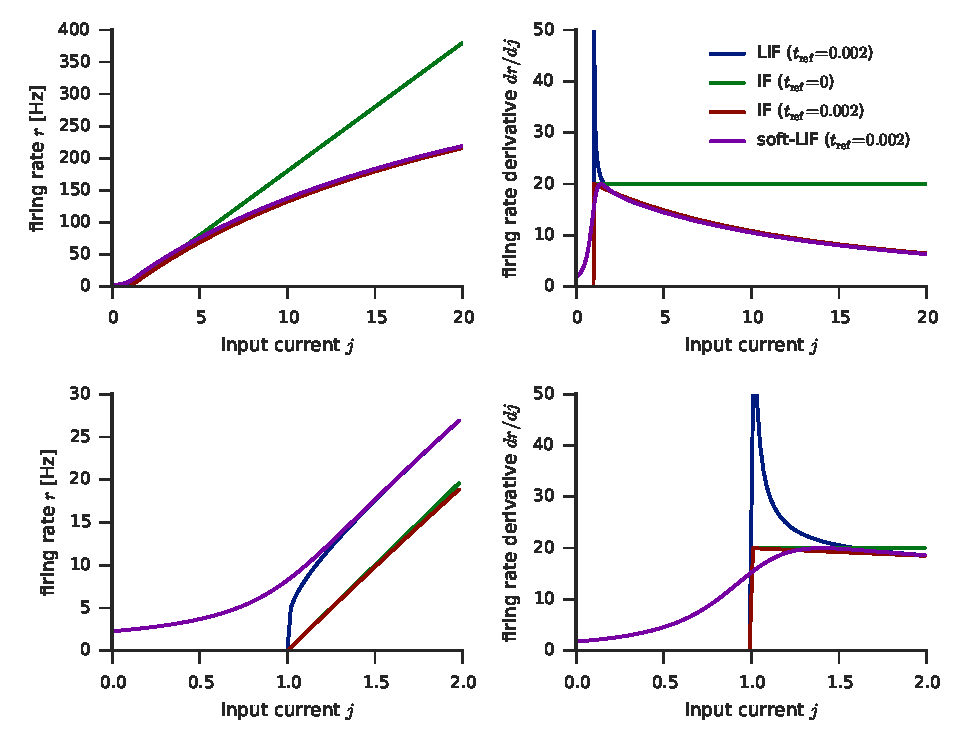
\includegraphics[width=\columnwidth]{derivative.pdf} \\
  \captionb{Comparison of neuron derivatives (right)
    and the response functions on which they are based (left).}{
    The top row shows the functions across a wide range of input currents.
    The bottom row shows their behaviour around the firing threshold.
  }
  \figlabel{learning-derivatives}
\end{figure}


\fig{learning-derivatives} shows three different neural response functions
and their corresponding derivatives.
Since the goal is to implement spiking networks in LIF neurons,
only the LIF response function is representative
of the firing behaviour of the neurons themselves,
but the singularity in the LIF response derivative around the firing threshold
prevents it from being used within a learning algorithm.
One option for a surrogate derivative function
is to simply use the LIF derivative function,
but with the value ``clipped'' to fall within a reasonable range.

The other functions shown in \fig{learning-derivatives}
can also be used as surrogate derivatives for LIF neurons.
The IF curve with no refractory period ($\tref = 0$)
is identical to the ReLU unit common in machine learning;
its derivative is simply a scaled step function.
The IF neuron with refractory period ($\tref = 0.005$)
introduces saturation in the firing rate.
Near the firing threshold, it acts linearly (as does the other IF curve),
but for larger input currents the firing rate saturates
and it approaches the LIF curve.
The derivative is qualitatively similar to that of the LIF neuron
everywhere except near the firing threshold,
where it does not suffer from the singularity present in the LIF neuron.
The equation for the IF curve is
\begin{align}
  r(j) = \left[\tref + \taurc \frac{1}{\rho(j - 1)}\right]^{-1}
\end{align}
where $\rho(x) = \max(x, 0)$ is the rectified linear function.
In contrast, the LIF curve is given by
\begin{align}
  r(j) = \left[\tref + \taurc \log\left(1 + \frac{1}{\rho(j - 1)}\right)\right]^{-1} \text{ .}
\end{align}
Since $\log(1 + x) \approx x$ for $x$ near zero,
for large values of $j$ the two curves become indistinguishable.
It is only around the firing threshold that the two functions behave differently.
The same is true of their derivatives, as shown in the figure.
Thus, the derivative of the IF curve with refractory period
is a good surrogate for the LIF derivative.

The soft-LIF neuron developed in the previous chapter
can also be used to provide a surrogate derivative for the LIF neuron.
By controlling the smoothing parameter $\gamma$,
we can control how closely the soft-LIF curve approximates the LIF curve;
larger $\gamma$ leads to a better approximation,
but also results in more extreme values in the derivative.
To facilitate comparison with the other derivative functions,
I chose $\gamma = 0.146$ such that the maximum value of the soft-LIF derivative
equaled the same maximum value as the other surrogate derivative functions.

% not addressing biological mechanisms of backpropagation
One aspect of this problem that I do not address here
are the biological mechanisms by which error or derivative information
may be transmitted within a neuron.
FA uses a three-factor learning rule,
with factors corresponding to the presynaptic neuron activity,
the derivative of the postsynaptic neuron activity,
and the projected error.
Since the postsynaptic neuron activity is based on all the incoming signals
to the postsynaptic neuron,
it is not locally available at the afferent synapses in question
without some process to transmit it back from the soma through the dendrites.
This is the function often credited to backpropagating action potentials,
which behave analogously to axonal (forward) action potentials,
but traveling backwards from the cell soma into the dendrites.
The postsynaptic neuron activity is something that is required
in many different learning rules, including all Hebbian and STDP-based rules.
To get this information to the synapses,
the backpropagating action potentials would have to be timed or transmitted
in such a way that they would not interfere with electrical currents passing
forward through the dendrites (from synapse to soma).
In this thesis, I am not modelling backpropagating action potentials explicitly,
thus I do not account for any of these potential interference effects.


\subsection{Spiking details}
\scnlabel{fa-spiking}

One of the main goals of this chapter is to implement FA
in a biologically plausible spiking network model.

% Limitations of Lillicrap spiking model
Along with the original presentation of the FA algorithm,
\textcite{Lillicrap2014} present a spiking implementation.
However, their model has a number of limitations:
\begin{enumerate}
  \item It does not use spiking neurons with a state,
    but rather uses sigmoidal neurons that spike stochastically
    with a probability given by the sigmoid function.
    This makes it significantly easier to find the neuron derivative.
  \item To represent both positive and negative feedback errors,
    the feedback path also uses neurons with a sigmoid response,
    but centred around zero and thus allowing negative firing rates.
    The authors justify this use of negative firing rates
    by referencing climbing fibres in the cerebellum,
    which fire tonically and raise or drop their firing frequency
    around this tonic rate to code positive or negative errors, respectively.
    They provide no evidence that cortical cells use such a coding scheme.
  \item The model consists of only a single hidden layer.
    This simplifies the timing problem,
    by limiting the maximum possible delay in the network.
    It also does not address issues around error transmission,
    since for one layer all FA variants (GFA, LFA, DFA) are equivalent.
\end{enumerate}

There are two subsequent papers---%
\textcite{Neftci2017} and \textcite{Samadi2017}---%
that address some of these issues in spiking neurons
(see \scn{fa-bg} for summaries).
Both use the direct variant of FA,
which is simpler to implement in spiking neurons
because it does not require mixing derivative information
into the feedback chain like GFA,
and also makes it easier to code both positive and negative errors
using nonlinear feedback neurons
due to the lower dimensionality of the error signal.

\begin{figure}
  \centering
  \tikzstyle{line} = [draw]

\begin{tabular}{c|c|c}
  BP & FA & My model \\
\begin{tikzpicture}[->,>=stealth',auto,node distance=1.2cm,
    thick,circnode/.style={circle,draw,inner sep=2}]
  \node[circnode] (h) {$h$};
  \node[circnode] (d) [right of=h, node distance=2cm] {$\delta$};
  \node[] (ah) [above of=h] {};
  \node[] (bh) [below of=h] {};
  \path[line] (bh) -- node [right] (W) {$W$} (h);
  \path[line] (h) -- (ah);
  \node[] (ad) [above of=d] {};
  \node[] (bd) [below of=d] {};
  \path[line] (ad) -- (d);
  \path[line] (d) -- node [right] {$W^T$} (bd);
  \path[line] (h) to [out=45,in=135] node {$h'$} (d);
  \path[line] (d) to (W);
\end{tikzpicture}
&
\begin{tikzpicture}[->,>=stealth',auto,node distance=1.2cm,
    thick,circnode/.style={circle,draw,inner sep=2}]
  \node[circnode] (h) {$h$};
  \node[circnode] (d) [right of=h, node distance=2cm] {$\delta$};
  \node[] (ah) [above of=h] {};
  \node[] (bh) [below of=h] {};
  \path[line] (bh) -- node [right] (W) {$W$} (h);
  \path[line] (h) -- (ah);
  \node[] (ad) [above of=d] {};
  \node[] (bd) [below of=d] {};
  \path[line] (ad) -- (d);
  \path[line] (d) -- node [right] {$B$} (bd);
  %% \path[line] (h.north) to [out=45,in=45] node {$h'$} (W);
  \path[line] (h.north) .. controls +(right:5mm) and +(up:5mm)
                        .. node {$h'$} (W.north east);
  \path[line] (d) to (W);
\end{tikzpicture}
&
\begin{tikzpicture}[->,>=stealth',auto,node distance=1.2cm,
    thick,circnode/.style={circle,draw,inner sep=2}]
  \node[circnode] (h) {$h$};
  \node[circnode] (d) [right of=h, node distance=2cm] {$e$};
  \node[] (ah) [above of=h] {};
  \node[] (bh) [below of=h] {};
  \path[line] (bh) -- node [right] (W) {$W$} (h);
  \path[line] (h) -- (ah);
  \node[] (ad) [above of=d] {};
  \node[] (bd) [below of=d] {};
  \path[line] (ad) -- (d);
  \path[line] (d) -- (bd);
  %% \path[line] (h.north east) to [out=45,in=45] node {$h'$} (W);
  \path[line] (h.north) .. controls +(right:5mm) and +(up:5mm)
                        .. node {$h'$} (W.north east);
  \path[line] (d) to node [below] {$B$} (W);
\end{tikzpicture}

\end{tabular}

  \captionb{Comparison of spiking architecture with FA and BP.}{
    The spiking architecture used here is identical to DFA,
    except that it uses an independent error population
    at each layer of the network.
    Since all the error populations encode the same output-layer error
    using population coding,
    this method is mathematically identical to DFA.
    However, it introduces a more biologically plausible delay structure
    into the network.
  }
  \figlabel{fa-spiking-arch}
\end{figure}

% Compare to Neftci methods
% - does not update in first 50 ms of digit presentation
% - update when pre-synaptic neuron spikes
The spiking network exhibited in this chapter is a type of DFA (\fig{fa-spiking-arch}).
While it shares a number of similarities with \textcite{Neftci2017},
it was developed independently \parencite{Hunsberger2017}.
There are notable differences between the two networks:
1) I use population coding to transmit the error backwards;
2) my network uses continuous learning,
whereas their network has a blackout period at the start of each stimulus presentation
when no learning occurs.

Rather than having only one error population,
I use population coding to transmit the error backwards
from each layer to the previous layer.
This is a more biologically plausible connection structure,
since it avoids many long range connections from the output layer
to each of the hidden layers.
In doing so,
it accounts for transmission delays in the feedback channel,
which biological networks have to overcome.
It also bears some similarities to LFA,
since the connections between feedback populations do appear roughly random,
though they are designed to ensure no error information is lost in the transmission.

The learning blackout period at the start of each stimulus presentation,
as employed by \textcite{Neftci2017},
ensures that no learning occurs while the network is in transition
and neuron spiking in the forward and backward pathways
is not yet reflective of the new stimulus and error.
This idea may have some biological support,
since if the error signal is internally generated (as it must be in biological systems)
then it would likely be triggered by the stimulus in some way.
Yet a biological system would not be able to turn off learning instantaneously;
there would still be residual activities in the neurons when a stimulus changes,
which may drive incorrect learning in the system for a brief time.
The network presented here uses continuous learning,
which results in slightly less efficient learning.

% How derivative is calculated
% - Right now I do ``cheat'' by using the sum of input currents. Make it so I
%   don't cheat (probably only using step function), have comparison.
% - need tolerance so that almost-zero activity is treated as zero
Both networks compute a neuron's local activity derivative
based on the current input to that neuron.
This has potential biological limitations,
since it is unclear how a specific synapse
would be able to use a derivative
that is dependent on the inputs to all synapses in the neuron.
It seems more plausible that the neuron derivative would be computed
based on the neuron output (spikes),
and the signal carried to the dendrites via backpropagating action potentials.
From a computational perspective,
this adds additional noise to the derivative signal,
and interferes with learning.
The networks presented here will use a derivative signal
computed on the total synaptic input to the cell,
as other implementations have.
Implementing a derivative based on spiking neuron output
remains an area of future work.


\subsection{Datasets}
\scnlabel{learning-datasets}

I use three different problems to evaluate the FA networks:
the \emph{linear} problem, the \emph{banded} problem, and the MNIST dataset.

In the linear problem,
the network has to learn a linear transform
from a higher-dimensional space to a lower-dimensional space.
Specifically, we have an $m \times n$ matrix of $m$ normally-distributed
$n$-dimensional input data points $\mat X$,
and our $d$-dimensional output targets are $\mat Y^* = \mat X \mat T$,
where $\mat T$ is an $n \times d$ matrix.
I orthogonalize the transform such that each dimension in the output space
corresponds to an orthogonal vector in the input space (\ie/ $T^T T = I$).
Learning is performed using a square cost (\ie/ MSE).
While this may sound like a trivial problem,
it is non-trivial for a network of non-linear neurons
to approximate a linear transform,
particularly if the neurons are nowhere linear (\eg/ LIF neurons or sigmoid neurons).%
\footnote{Since rectified linear units (ReLUs), also known as IF neurons,
  are linear above the firing threshold and silent below,
  two such neurons can perfectly fit a line (with appropriate weights).
  Therefore, networks of these neurons can solve the problem exactly.
  A network with one hidden layer would need $2d$ of these neurons
  for the exact solution.}
When training on this dataset,
I continuously generate new input-output pairs
during training using the transform.
Since no example is seen more than once,
the error during training is an unbiased measure
of the generalization (testing) error.

\begin{figure}
  \centering
  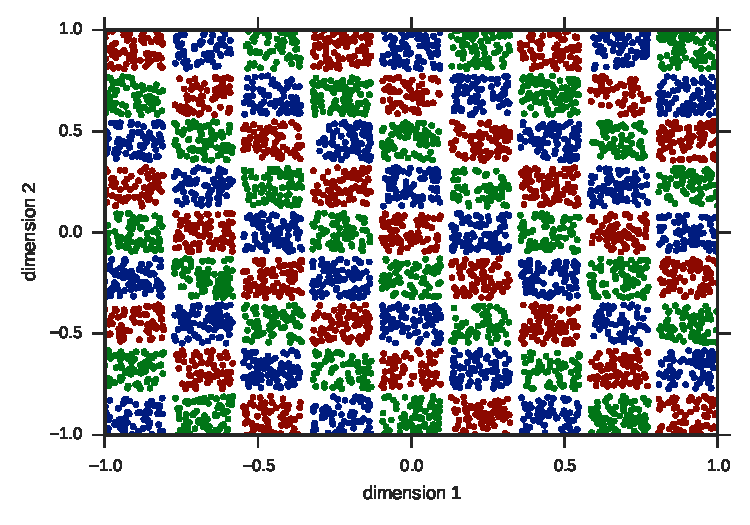
\includegraphics[width=5in]{banded2d_dataset.pdf}
  \captionb{Samples from the \dd/ banded dataset.}{
    The colours of points denote to which of the three categories they belong.
    Looking at only a single dimension gives no information
    about the class to which a point belongs
    (\ie/ the marginal distributions for all classes are identical).
  }
  \figlabel{banded-dataset}
\end{figure}

In the banded problem (\fig{banded-dataset}),
the data is arranged into bands in each dimension,
and the class of a datapoint is determined by which band it is in.
The mapping from bands to classes can be chosen such that
a single dimension contains no information about the class of a point;
only by using both dimensions can the class be determined (see \fig{banded-dataset}).
I will use this fact to help me distinguish some of the key differences
between different learning algorithms,
in terms of what kind of data distributions they are and are not suited to learn.

As a more challenging and realistic learning problem,
I use the MNIST dataset (\scn{datasets}).


\section{Results}

Since FA is still a relatively new algorithm,
there are many aspects of it that have not been well explored.
My goal with this chapter is to create a spiking model of FA learning,
in order to investigate whether the FA algorithm is a biologically plausible method
by which the brain may perform deep learning.
Before presenting the spiking model, however,
I first present some supporting results
to help justify my spiking architecture (see \scn{fa-spiking}),
including results comparing the different FA variants
and the different possible choices for the LIF neuron derivative.
I then present a fully spiking implementation
of the modified DFA algorithm (see \scn{fa-spiking})
using LIF neurons.
All rate-based experiments use the LIF rate nonlinearity
unless otherwise noted.

Throughout these results, I have made an effort to choose hyperparameters
such that BP and FA are directly comparable.
As noted in \scn{fa-parameters},
the scale of feedback weight matrices in FA can have
a very large effect on algorithm performance and learning rate,
since it can have an identical effect to setting individual learning rates
for each hidden layer.
To this end, I try to choose the overall learning rate
such that BP performs as well as possible.
Then, I choose the scale of the feedback matrices for FA
such that it performs as well as possible,
using the same overall learning rate as with BP.
This helps ensure that neither algorithm has an unfair advantage over the other
simply by having better-tuned learning rates.\footnote{
A better approach would be to use a hyperparameter optimization method
to find the ideal parameters for each algorithm,
but that is significantly more time-consuming.}


\subsection{FA variants}
\scnlabel{fa-variants-results}

I compared the performance of the different FA variants
(GFA, LFA, and DFA; see \scn{fa-variants})
on both the linear transform and MNIST learning tasks,
to look for differences between the algorithms in performance and stability.

\begin{figure}
  \centering
  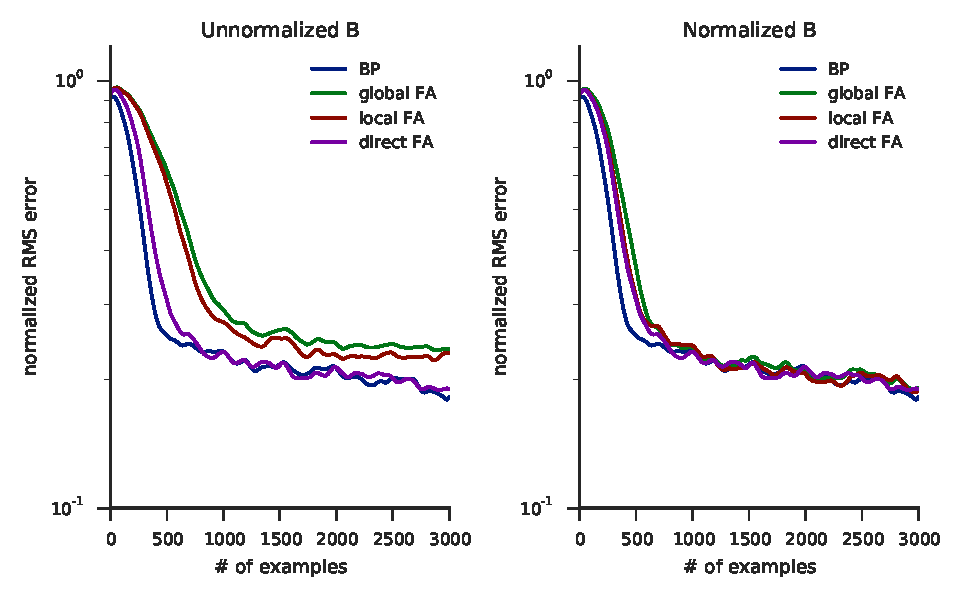
\includegraphics[width=6.35in]{variants_offline_linear.pdf}
  \captionb{Comparison of FA variants on the linear-transform problem.}{
    In the left panel,
    all feedback ($\mat B$) matrices have been generated to have the same norm (0.2).
    However, this gives larger-magnitude errors in the early layers of direct FA
    as compared to global and local FA,
    since their early-layer errors are the result
    of passing through multiple $\mat B$ matrices.
    In the right panel, the $\mat B$ matrices have been normalized so that the
    early-layer errors in GFA and LFA will have the same magnitude as with DFA.
    In this situation, we see that the variants all perform comparably.
  }
  \figlabel{variants-linear}
\end{figure}

\fig{variants-linear} shows the results on the linear transform problem.
It looks at two cases:
The first is where all $\mat B$ matrices have the same norm
across all different variants of FA.
However, since GFA and LFA both pass the output error through multiple
$\mat B$ matrices when propagating it to earlier hidden layers,
having a matrix norm less than one can mean that the magnitude of the error signal
becomes significantly smaller in earlier layers.
This can be seen in the results, where the GFA and LFA algorithms
both learn significantly slower than DFA and BP.

To account for this, I looked at a second case where
I normalized the magnitudes of the $\mat B$ matrices for the GFA and LFA algorithms,
such that the combined magnitudes of the $\mat B$ matrices
leading back to a given hidden layer
equals the magnitude of one of the $\mat B$ matrices in the DFA algorithm.
This ensures that the magnitudes of the errors at each hidden layer
are approximately the same.\footnote{
  This assumes a linear feedback path, which is the case for LFA,
  but not for GFA.
  Since GFA has the hidden unit derivatives included in the feedback path,
  the feedback error will be slightly smaller,
  since some of the hidden units at each layer are off and thus silence
  the corresponding element of the error signal.
  For this experiment, I used a step derivative function,
  and chose the feedforward amplitude on the LIF neurons
  such that the derivative equals one when the neuron is active.
  This allows GFA to be comparable to DFA and LFA,
  since the derivative does not have a scaling effect on the error,
  other than to silence some elements.}
With these normalized weights,
all the FA algorithms learn quite comparably on the linear problem,
and perform similarly to BP.
It is interesting to note that the inclusion of the neuron derivatives
in the feedback pathway does not appear to benefit GFA,
despite these same derivatives playing an important role in the BP algorithm.
This suggests that GFA is not making use of these derivatives in any
meaningful way,
due to the lack of correspondence between
the role that each neuron plays in the feedforward network computation
and randomly-projected error signal that drives the learning.


\begin{figure}
  \centering
  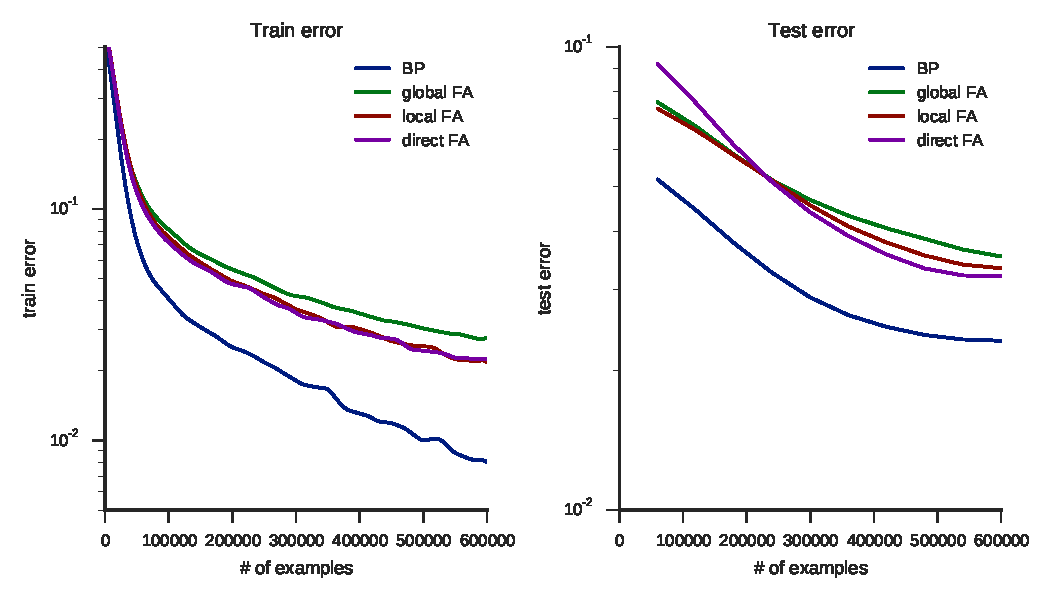
\includegraphics[width=6.35in]{variants_offline_mnist.pdf}
  \captionb{Comparison of FA variants on the MNIST dataset.}{
    The FA variants perform similarly on MNIST.
    GFA learns slightly slower,
    because the neural derivatives in the feedback pathway
    set some error components to zero
    (this experiment uses a step function as the surrogate derivative,
    scaled so that the output is unity if the neuron is active).
  }
  \figlabel{variants-mnist}
\end{figure}

To better understand whether there are performance differences
between the FA variants and BP,
I also compared them on the MNIST dataset (\fig{variants-mnist}).
This dataset is more challenging,
and shows more difference between the algorithms.
First, BP significantly outperforms all the FA variants,
scoring significantly better on both the training and test sets.
The FA results depend on the run;
a specific randomly-generated feedback matrix can be responsible
for considerable changes in performance,
particularly generalization performance.
One result that is consistent, however,
is the rate at which the training error decreases for different FA variants.
DFA and LFA both show similar rates of training error decrease,
and are faster than the decrease shown by GFA.
This is because GFA reduces the magnitude of the error signal
by multiplying by the neural derivatives
(which for this experiment are given by a step function that outputs zero or one),
while LFA and DFA do not.


\begin{figure}
  \centering
  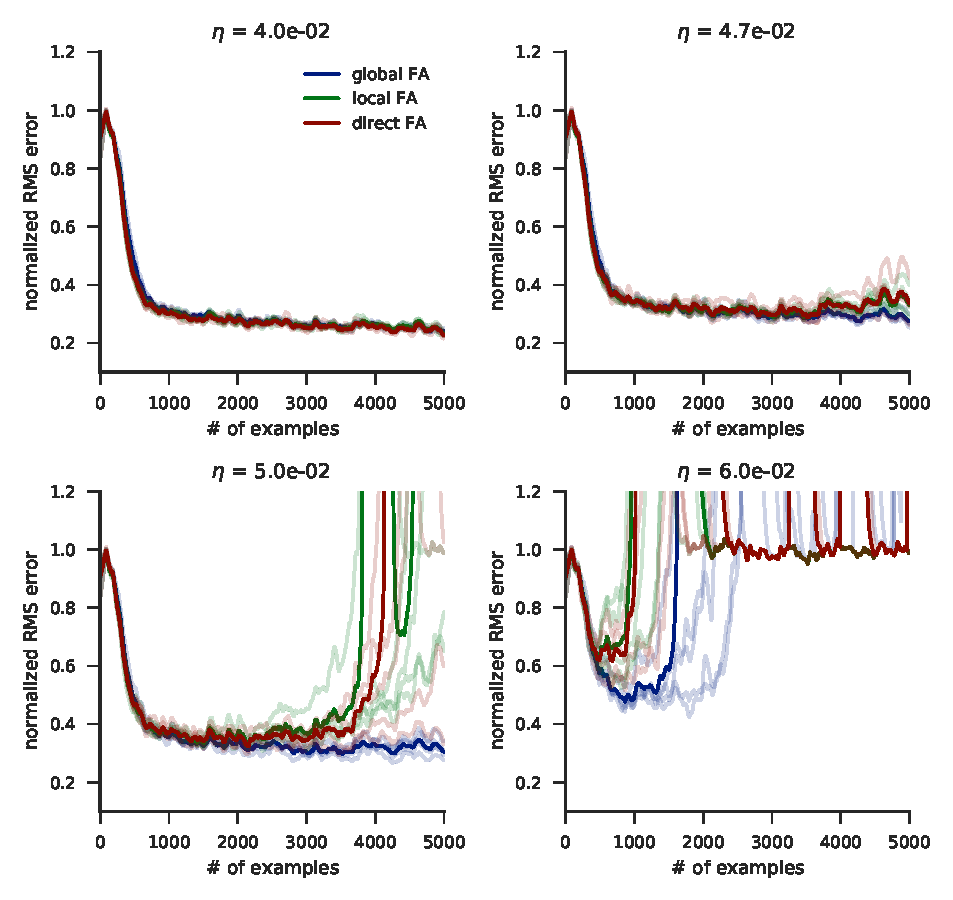
\includegraphics[width=6.35in]{variants_offline_linear_critical.pdf}
  \vspace*{-2.5em}
  \captionb{Comparison of FA variant stability on the linear-transform problem.}{
    To evaluate FA variant stability,
    this figure compares the three variants with different learning rates.
    At the lowest rate ($\eta = 0.04$), all the variants are stable.
    At the moderate rate ($\eta = 0.05$), LFA and DFA lose stability,
    but GFA is still marginally stable.
    At the highest rate ($\eta = 0.06$), all are unstable.
    What is noteworthy is that these learning rates are so close together,
    suggesting that GFA does not significantly improve stability.
    The fact that it is slightly more stable is likely simply because
    the derivative terms in the error set some values to zero,
    making the overall magnitude of the projected error smaller.
  }
  \figlabel{variants-stability}
\end{figure}

Despite being slightly slower to learn than LFA and DFA,
it is possible that GFA is more stable
because it keeps the derivative in the feedback chain.\footnote{
  I investigated a local variant of BP,
  where the derivative is not used in the feedback chain,
  and found that it is significantly less stable than ordinary BP.}
To test this, I investigated the three FA variants with learning rates
around the point at which the algorithms begin to lose stability.
I used the linear problem,
and as before, I scaled the amplitude of the LIF neurons
so that when using a step derivative,
it would output one if the neuron is active and zero if silent,
thus not scaling the error for active neurons.
As shown by \fig{variants-stability},
when the overall learning rate $\eta = 0.04$,
all three algorithms are stable.
Increasing $\eta$ to 0.05 causes LFA and DFA to lose stability, but not GFA.
Increasing $\eta$ again to 0.06 causes GFA to lose stability as well.
Thus, GFA loses stability at a slightly higher learning rate than LFA and DFA
(on the linear problem).
However, this can be explained by the fact that the error signal in GFA is
slightly smaller,
since some of the error elements are zeroed by the derivatives.
My conclusion is that GFA is not inherently more stable than LFA or DFA,
and there is no benefit to using the derivatives in the feedback pathway.


\subsection{Derivatives}
\scnlabel{fa-derivatives-results}

\begin{figure}
  \centering
  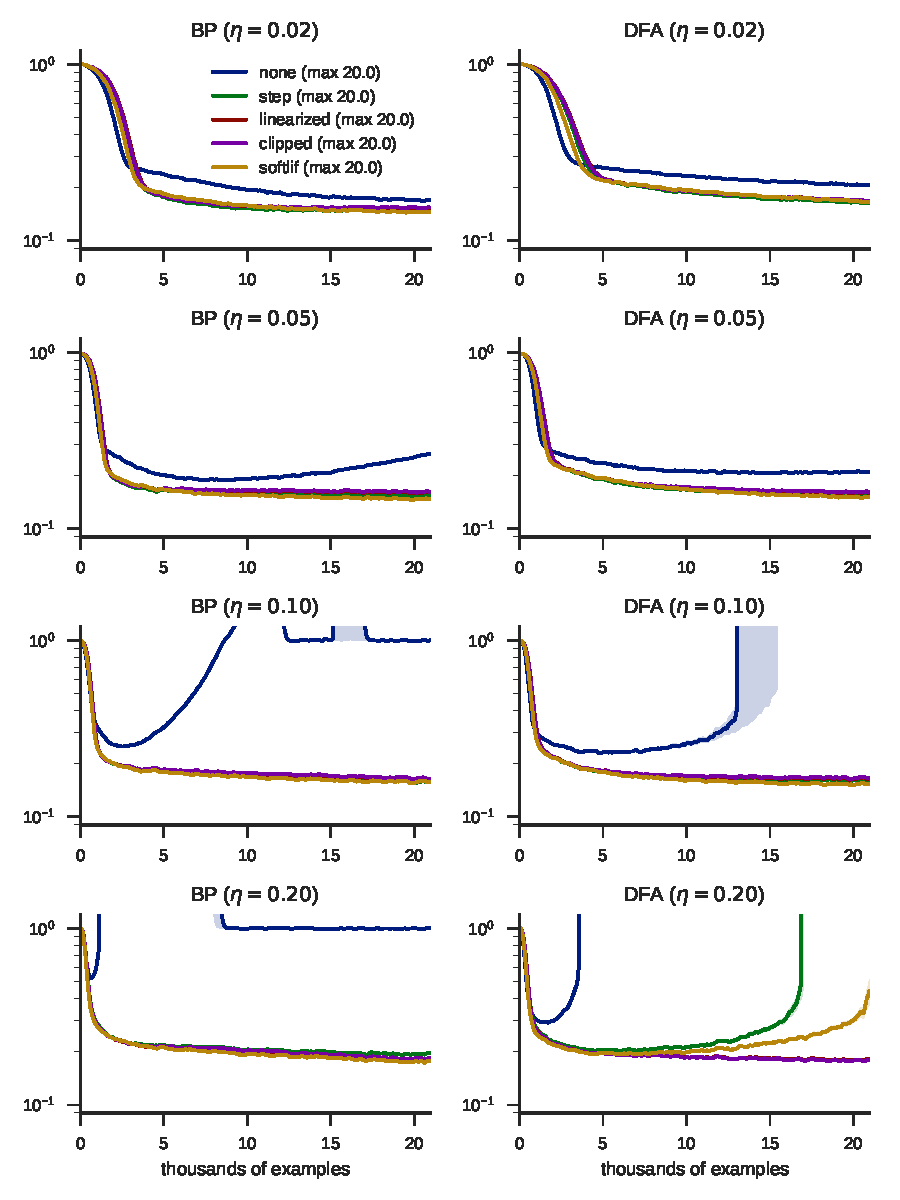
\includegraphics[height=6.4in]{derivative_offline_linear_multi.pdf}
  \captionb{Comparison of alternative neuron derivatives on the linear problem.}{
    The left column shows BP performance, the right column FA performance.
    Having no derivative (``none'') causes significant stability problems
    for both BP and DFA.
    The other derivatives perform similarly,
    except with high learning rates with DFA,
    where the step and soft-LIF derivatives lose stability
    before the clipped LIF and IF (``linearized'') derivatives.
  }
  \figlabel{derivative-offline-linear}
\end{figure}

\fig{derivative-offline-linear} compares different LIF surrogate derivatives
on the linear problem.
I normalized all derivatives to have the same maximum value,
to reduce effects due to one derivative simply having a larger magnitude than another
(see \fig{learning-derivatives} for an illustration of the derivatives).
For BP (left column), having no derivative (``none'')
leads to qualitatively different results than all of the surrogate derivatives.
Even at low learning rates ($\eta = 0.02$),
where the no derivative option appears stable,
it still learns considerably more slowly.
It becomes unstable even at moderate learning rates ($\eta = 0.05$).
The same is the case for FA, where having no derivative is unstable
at $\eta = 0.1$.

The other derivatives all appear equally stable when used with BP,
and learn equally well.
The same is true with FA across most learning rates.
At the highest learning rates, which begin to test the algorithm's stability,
the step-function derivative becomes unstable first,
followed by the soft-LIF derivative.
The clipped LIF derivative and IF derivative (``linearized'')
show the best stability and learning characteristics,
performing equally well across all the test cases.
A careful examination of the behaviour at the smallest learning rate
shows that in that case,
the soft-LIF derivative is able to learn slightly faster
than the other derivatives;
this is possibly because it is non-zero just below the firing threshold,
thus helping neurons on the verge of firing to get involved.

\begin{figure}
  \centering
  \includegraphics[width=6.35in]{{derivative_offline_mnist_multi_eta=0.020_log}.png}
  \captionb{Comparison of alternative neuron derivatives on the MNIST dataset.}{
    Again, having no derivative is problematic to learning.
    All other derivatives perform similarly with BP,
    but with FA the step derivative performs slightly worse.
  }
  \figlabel{derivative-offline-mnist}
\end{figure}

\fig{derivative-offline-mnist} shows a similar experiment using the MNIST dataset.
Again, using no derivative is clearly detrimental to learning.
More surprisingly, the step derivative function
performs as well as other derivative functions when used with BP,
but slightly worse than the others when used with FA.
Overall, FA performs worse than BP in terms of both training and testing error.


\subsection{Selectivity}
\scnlabel{fa-selectivity-results}

One of my hypotheses for how FA works
is that the random feedback weights
push neurons to be selective for different categories.
I investigated this hypothesis by looking at
the correlation between a neuron's feedback weights $\mat B^i$
and its activity in response to stimuli of each different class.
To do this, I trained a 784-500-500-10 network on MNIST.

\begin{figure}
  \centering
  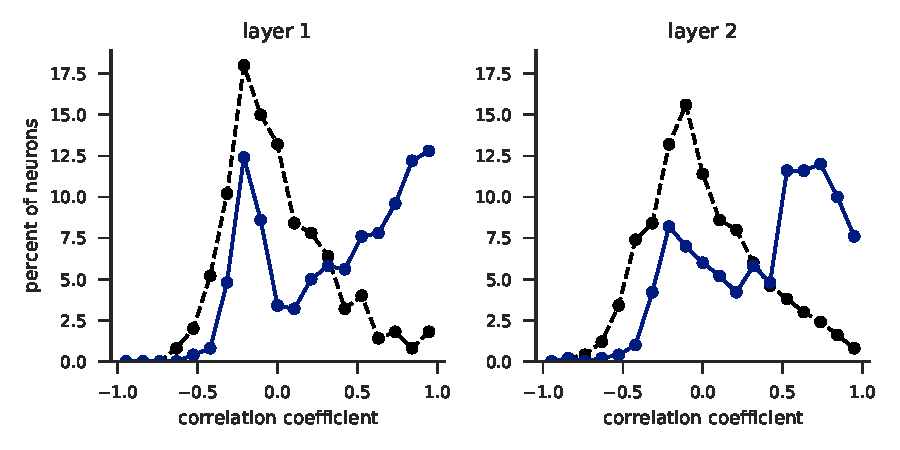
\includegraphics[width=6in]{selectivity_offline_mnist_corrhist.pdf}
  \captionb{Correlation between neural activities and feedback weights.}{
    Histograms of correlation coefficients between
    the vector of a neuron's mean activity
    across stimuli from each different class
    and its feedback vector,
    for the two hidden layers of a 784-500-500-10 MNIST network.
    Dashed lines show the initial (random) weights,
    solid lines show after training with DFA.
    The activity and feedback vector are generally positively correlated
    after training,
    indicating that DFA does push neurons to be more selective
    for particular classes over others.
  }
  \figlabel{selectivity-corr}
\end{figure}

\fig{selectivity-corr} shows the correlation between
the feedback weights for a neuron
and the pattern of activity for that neuron across classes
(in a DFA network).
The post-training histogram of correlation coefficients is skewed significantly
to the positive side for both layers,
suggesting that FA does push neurons to be selective for particular classes.
The shift from before to after training is also clearly positive.
Yet the correlation between activity and feedback vector is not perfect.
This is indicative of the fact that neuron weights are only updated
when there is an error.
So for example, if the network is able to learn to classify the digit ``1''
(one of the easier digits to distinguish)
early on in the training,
then there will be few errors on 1s,
and neurons that are mostly tuned to that digit
will have fewer changes in weights.
Also, some neurons may be ``naturally'' tuned (based on their initial feedforward weights)
to a set of digits completely different than what their feedback weights
are pushing them towards.
Such neurons may end up with activities that are more correlated
with their feedback weights,
but may never become strongly correlated.


\subsection{Limitations}
\scnlabel{fa-limitations-results}

As described previously (\scn{fa-intuitions}),
one intuition for what FA is doing
is that the feedback weights are pushing the hidden neurons
to each be selective to different output classes,
thus making them useful for decoding class information.
This has an apparent limitation:
if hidden neurons in a particular layer
do not have the information that they need
to be selective for one class over another,
then pushing them to be selective for some classes
is simply going to push them in random directions.
To both illustrate and demonstrate this limitation,
I have designed a network where this is the case.
For this, I use the \dd/ banded dataset (see \scn{learning-datasets}),
which has the property that class information can only be determined
using both input dimensions.\footnote{
  Put another way, the marginal distributions across either input dimension
  contain no class information.}
Using this dataset, and limiting each first-layer neuron to only receive input
from one input dimension or the other,
results in a problem that BP is able to solve but FA is not.
For simplicity, this experiment uses ReLU neurons.

\begin{figure}
  \centering
  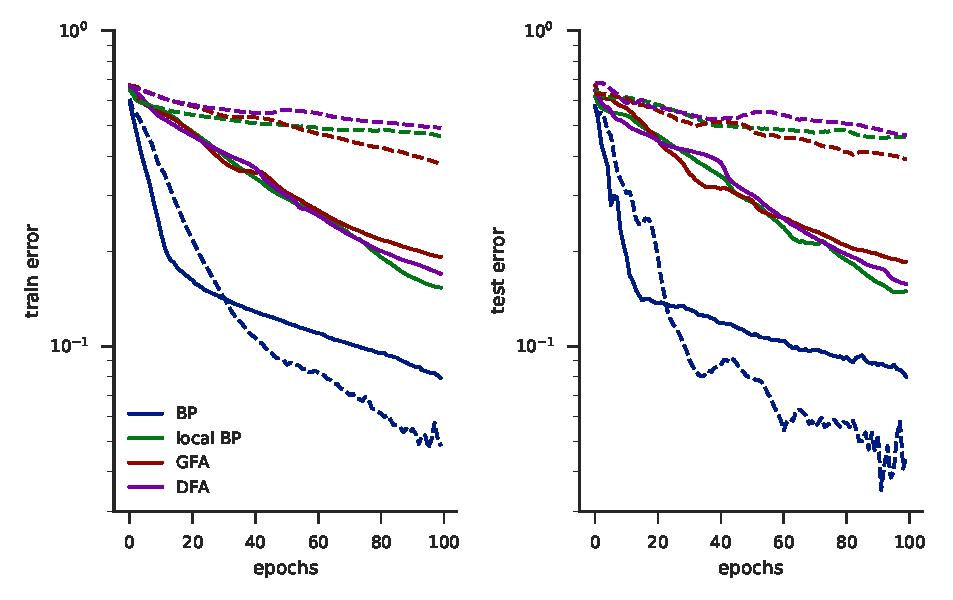
\includegraphics[width=6.35in]{banded2d_losses.pdf}
  \captionb{Comparison of learning methods on the \dd/ banded dataset.}{
    The solid lines show the fully-connected case,
    where first-layer hidden neurons are connected to both input dimensions.
    The dashed lines show the limited-connectivity case,
    where each first-layer hidden neuron connects to
    only one of the two input dimensions or the other.
    Learning is impaired in the limited-connectivity case for
    GFA, DFA, and local BP, but not for standard BP.
  }
  \figlabel{banded2d-comparison}
\end{figure}

The upper panel of \fig{banded2d-comparison}
shows the experiment where the input (first-layer) weights are unconstrained;
that is, first-layer hidden neurons can receive input from both input dimensions.
In this case, both BP and FA are able to learn.
BP still outperforms FA on the task, though;
this is because the number of neurons in the first layer
is too low for FA to have one neuron per section on the grid.
In the constrained case,
where each first-layer neuron only receives input
from one of the two input dimensions,
we see that FA performs much worse.
This suggests that FA is unable to properly solve the credit assignment problem
to learn hierarchically.
BP, on the other hand, \emph{is} able to learn hierarchically,
and performs better.

% Fact that local BP also does poorly reflects importance of
% derivative in feedback chain
It is surprising that local BP---%
that is, BP with the neuron derivatives only applied locally,
but not included in the feedback pathway---%
is also not able to solve the problem.
This suggests that the neuron derivatives are an important part
of the credit assignment process,
and not including them in the feedback pathway is detrimental.
Unfortunately, there is no obvious way to include the neuron derivatives
in FA in a useful manner.
As seen previously, and as evidenced by the poor performance of GFA on this task,
simply including the neuron derivatives in the feedback pathway (in a similar manner to BP)
is not helpful.


\subsection{Adaptive variants}

\begin{figure}
  \centering
  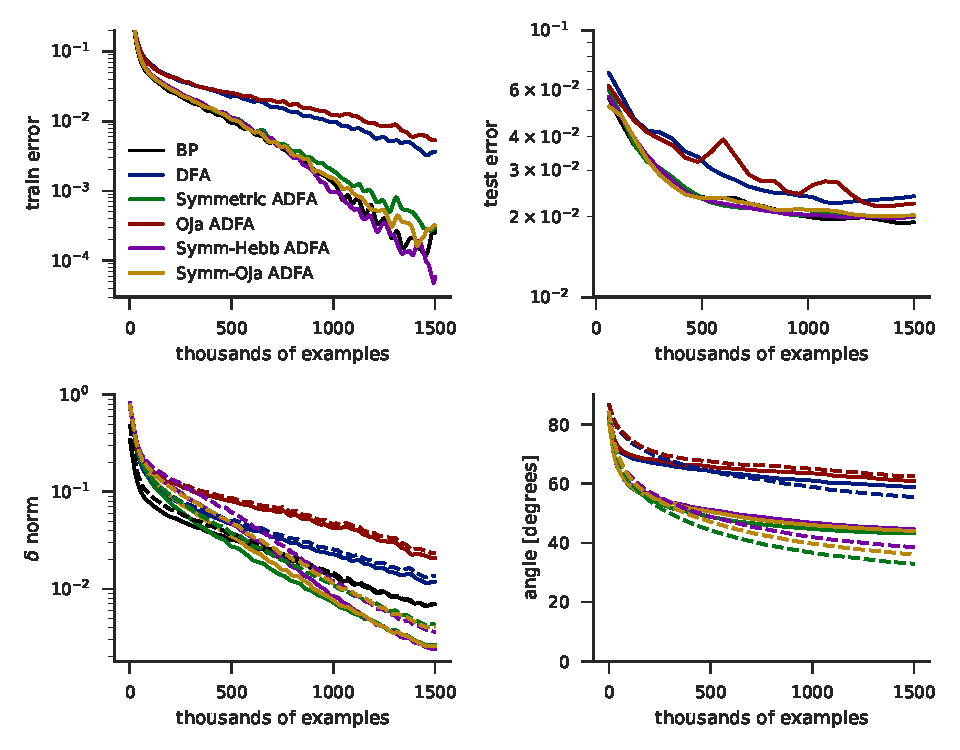
\includegraphics[width=6.35in]{adaptive_offline_mnist.pdf}
  \captionb{Comparison of adaptive variants on MNIST task.}{
    The top-left and top-right panels show the training error and testing error, respectively.
    The ability to decrease training error
    is the best reflection of each algorithm's performance.
    The bottom-left panel shows the magnitude of $\delta$,
    where $\delta$ is the projected error times the local neuron derivative.
    The bottom-right panel shows the angle between the actual (FA) update
    and the ideal (BP) update.
    In the bottom plots, solid lines show the first hidden layer,
    and dashed lines show the second hidden layer.
    For all variants, $\mu = 1.0$ and $\nu = 0.1$;
    thus the symmetric component of the adaptation
    has the same learning rate as the forward weights,
    whereas the unsupervised component (Hebbian or Oja) has one-tenth the learning rate.
    This is required for stability.
  }
  \figlabel{adaptive}
\end{figure}

I compared the performance of adaptive variants of DFA (the ADFA variants)
on the MNIST task.
Preliminary experiments indicated that the Hebbian and Oja variants
offered a performance improvement over non-adaptive DFA.
A closer examination of this result
revealed that the magnitude of the feedback weights
was smaller than optimal,
and that the benefit from these adaptive variants
was because they increased the magnitude of these weights,
thus speeding up convergence.

\fig{adaptive} shows the revised experiment
with closer to optimal feedback weight magnitude.
In this case, the Oja variant no longer performs better than DFA;
in fact, it performs slightly worse.
As in the preliminary experiments,
the Oja variant increases the $\delta$ magnitudes (and thus the learning rate),
but in this situation,
the original (unadapted) $\delta$ magnitudes were near-optimal,
and increasing them is only detrimental.
Additionally, the angles between the Oja ADFA updates
and the ideal BP updates are worse than for DFA,
thus the adaptation is not pushing the weights in a useful direction.
The Hebbian variant is not shown,
because it becomes unstable in this experiment,
even though its learning rate is one-tenth the forward learning rate ($\nu = 0.1$).

Symmetric ADFA does considerably better than DFA,
with performance nearing that of BP.
The angle between the symmetric ADFA updates and BP
is much better than the DFA angles,
since the updates are pushing both the forward and backwards weights
in the same direction, aligning them.
The combined Symmetric-Hebbian and Symmetric-Oja variants
also perform well.
Near the end of training,
their performance appears to surpass that of Symmetric ADFA,
though it is unlikely that this result is significant.


\subsection{Spiking network}
\scnlabel{fa-spiking-results}

\begin{figure}
  \centering
  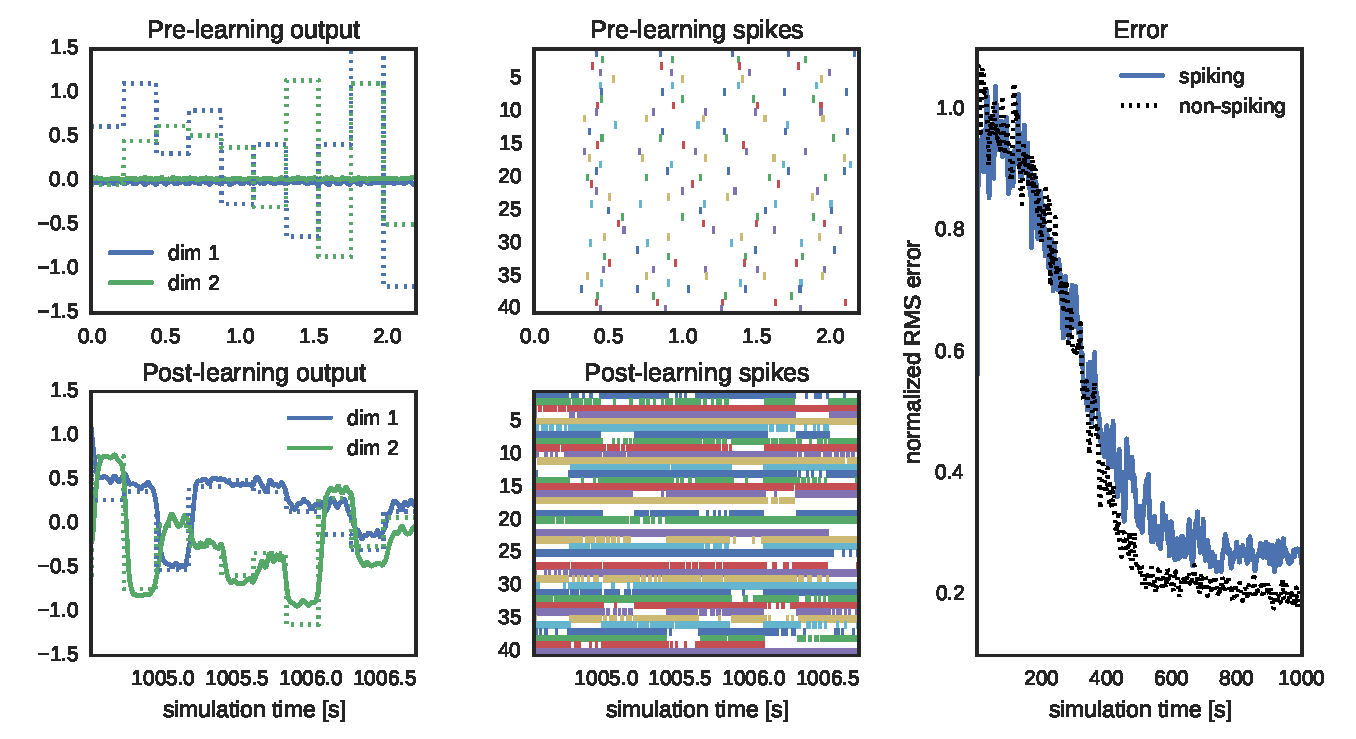
\includegraphics[width=\columnwidth]{../cosyne_poster/figures/online.pdf}
  \captionb{Spiking network learning the linear problem.}{
    The left panels show the network output (solid traces)
    as compared with the desired output (dotted traces)
    before and after learning.
    The centre panels shows the spiking of the first hidden layer
    before and after training.
    The right panel shows the overall error rate of the spiking and rate
    networks during the course of training.
  }
  \figlabel{online-overview}
\end{figure}

A summary of the online spiking learning system is shown in \fig{online-overview}.
The system learns to perform the linear task.
The top panels show the performance of the network before learning;
there is a minimal, uniform response to all stimuli,
and the neuron spiking is sparse and does not seem to be indicative
of what stimulus is present.
The bottom panels show the performance after learning, on novel test stimuli.
The network output matches the target output values well,
and the neurons are both more active,
and appear to be selective to specific regions of the input space.
As shown by the far-right panel,
the error of the spiking network
decreases to almost the same level as that of the network trained offline.

% important factors when training spiking networks
% - presentation time for each example
% - total training time
% - learning rate
% need to balance number of examples seen (shorter pt -> better) with
% sufficient time on each example for the network to settle and learn.
% Also a tradeoff between faster learning on each example (longer pt, larger lr)
% and good learning for generalization \ie/ not overfitting/forgetting (shorter pt, smaller lr)
% Presentation time also related to learning rate,
% since larger LR will mean more forgetting of past stimuli, need quicker succession of stimuli
When learning in online spiking networks,
there are a number of different factors that affect
how well the network learns.
As with non-spiking networks,
the learning rate has a strong effect on how well the network learns.
While larger learning rates theoretically
allow the error to decrease more quickly,
if the learning rate is too large,
then the network will fit itself too much to each new stimulus,
and lose some of the information learned from previous stimuli.
This problem is more acute in online learning,
since each stimulus is shown for multiple time steps,
giving the network more time to overfit to the new stimulus.
I found that if the system is able to reduce the error to close to zero
on each new stimulus presentation, particularly during early learning,
this indicates the learning rate is too large.
Optimal learning rates showed only a slight decrease in error
over the course of each stimulus presentation,
but after many such presentations,
the network was able to learn the desired function quite well.

The presentation time for each stimulus also has a large effect on learning.
Assuming the total training time is fixed,
there is a tradeoff between showing each stimulus for a long time
and showing many stimuli.
Each stimulus must be shown for an adequate length of time to learn well,
since at the onset of each new stimulus there are considerable transients
due to past information stored in synapses and membrane voltages.
It is only once the network has settled into its feedforward state
that useful learning can occur.
However, if stimuli are shown for too long,
this decreases the number of different stimuli that can be shown
in the allotted time,
limiting the diversity that the network is exposed to and
thus reducing its generalization performance.

Finally, the total training time affects performance.
While the basic relationship is that longer training times
mean exposure to more stimuli for longer times and thus better performance,
the outcome does depend on the learning rate and presentation time.
For example, if the presentation time is long or the learning rate is high,
then increasing the total training time may not improve performance
beyond a certain point.
In this situation, the network is constantly re-fitting itself
to the most recent stimuli and forgetting the old stimuli,
so increasing the total training time will only
increase the list of forgotten stimuli.


\section{Discussion}

% FA is not perfect at doing credit assignment; some problems it can't solve.
%   Is this a showstopper, though? How much credit assignment is needed in the brain?
%   Earlier visual areas are likely trained with other objective functions,
%   not just classification as currently happens.
% - Need for synchronization between forward and backward passes might also
%   limit the maximum depth for single-objective-function learning in the brain.
One limitation of Feedback Alignment (FA)---%
and a key difference with backpropagation (BP)---%
is that FA does not truly solve the spatial credit assignment problem.
Theoretically, this is most apparent in the case of direct FA,
where all hidden neurons only receive error information from the output layer.
Since they do not receive error information from any downstream neurons (\cf/ BP),
there is no way that they can update to reduce downstream errors,
they can only try to reduce the output error directly.
Since global FA and local FA essentially reduce to direct FA\footnote{
  Local FA is mathematically equivalent to direct FA,
  and global FA is the same as local FA
  but with an essentially random perturbation (the derivative scaling)
  on the feedback errors. See \scn{fa-variants}.},
they also face the same problem.
I confirmed this empirically with the experiments in \scn{fa-limitations-results}:
In the case of the \dd/ banded problem,
where no class information is available to the first layer neuron
it is impossible for FA to learn.
FA relies on pushing all hidden neurons to be selective
for some classes over others,
rather than reducing downstream hidden-neuron errors as BP does.
The result is that there are certain problems that are unlearnable by FA.

To determine whether this limitation of FA is a serious problem,
the next question should be: ``How much credit assignment is required in a brain?''
In the human visual system,
it is quite unlikely that classification error
is the only error signal available to the system.
Not only do earlier visual layers likely learn at least partly
based on features more associated with the dorsal stream (such as depth and motion),
but there is likely unsupervised learning happening at many layers.
Therefore, the amount of supervised deep learning that occurs in the brain
is almost certainly not as all-inclusive as is the case
in the models presented here.
Thus, the fact that FA can only learn when class information is available
may not be a serious limitation:
early visual layers---where there is typically less class information---%
could learn predominantly based on other signals,
with FA taking a leading role at the higher layers of the ventral stream
where more class-specific inputs are readily available.

%%  LocalWords:  Marblestone bp biomechanisms bg dtp Bengio nef Baldi
%%  LocalWords:  Grossberg Guergiuev Bogacz Balduzzi Lillicrap
%%  LocalWords:  Liao Ioffe Nokland DFA IFA ARBP ASRBP Neftci Samadi
%%  LocalWords:  ep Scellier RBP ij GFA qj LFA lj li mnist multi DNNs
%%  LocalWords:  unlearnable backprop ADFA Symm Hebb softlif
%%  LocalWords:  unadapted
